%Copyright 2014 Jean-Philippe Eisenbarth
%This program is free software: you can 
%redistribute it and/or modify it under the terms of the GNU General Public 
%License as published by the Free Software Foundation, either version 3 of the 
%License, or (at your option) any later version.
%This program is distributed in the hope that it will be useful,but WITHOUT ANY 
%WARRANTY; without even the implied warranty of MERCHANTABILITY or FITNESS FOR A 
%PARTICULAR PURPOSE. See the GNU General Public License for more details.
%You should have received a copy of the GNU General Public License along with 
%this program.  If not, see <http://www.gnu.org/licenses/>.

%Based on the code of Yiannis Lazarides
%http://tex.stackexchange.com/questions/42602/software-requirements-specification-with-latex
%http://tex.stackexchange.com/users/963/yiannis-lazarides
%Also based on the template of Karl E. Wiegers
%http://www.se.rit.edu/~emad/teaching/slides/srs_template_sep14.pdf
%http://karlwiegers.com
\documentclass{scrreprt}
\usepackage{listings}
\usepackage{underscore}
\usepackage{graphicx}
\usepackage{grffile}
\usepackage{svg}
\usepackage{makeidx}


\usepackage[bookmarks=true]{hyperref}
\usepackage[utf8]{inputenc}
\usepackage[english]{babel}
\hypersetup{
    % bookmarks=false,    % show bookmarks bar?
    pdftitle={Development Documentation},    % title
    pdfauthor={Mahmoud Khaled},                     % author
    pdfsubject={Relevium SRS},                        % subject of the document
    pdfkeywords={Project, Relevium, SRS}, % list of keywords
    colorlinks=true,       % false: boxed links; true: colored links
    linkcolor=blue,       % color of internal links
    citecolor=black,       % color of links to bibliography
    filecolor=black,        % color of file links
    urlcolor=purple,        % color of external links
    linktoc=page            % only page is linked
}%
\def\myversion{0.5}
\date{\today}
%\title
\usepackage{hyperref}

\makeindex
\begin{document}

\begin{flushright}
    \rule{16cm}{5pt}\vskip1cm
    \begin{bfseries}
        % \Huge{SOFTWARE REQUIREMENTS\\ SPECIFICATION}\\
        \Huge{DEVELOPMENT DOCUMENTATION}\\
        % \vspace{1.9cm}
        \vspace{1cm}
        for\\
        % \vspace{1.9cm}
        \vspace{1cm}
        % $<$Project$>$\\
        Relevium\\
        % \vspace{1.9cm}
        \vspace{1cm}
        \LARGE{Version \myversion}\\
        % \vspace{1.9cm}
        \vspace{1cm}
        % Prepared by $<$author$>$\\
        Prepared by\\
        Abd Elrahman Solyman - 
        Ahmed Samir \\
        Mahmoud Khaled -
        Mohamed ELTorky \\ 
        Mohamed Fathallah -
        Omar Mohamed\\
        
        \vspace{1cm}
        Supervised by\\
        Dr. Mohamed Magdy

        \vspace{1.2cm}
        % $<$Organization$>$\\
        % Arab Academy for Science, Technology \& Maritime Transport\\
        College of Computing \& Information Technology\\
        \vspace{1.2cm}
        \today\\
    \end{bfseries}
\end{flushright}

\tableofcontents
\begingroup
\let\clearpage\relax
\listoffigures
\endgroup


\newpage


\chapter*{Revision History}

\begin{center}
    \begin{tabular}{|c|c|c|c|}
        \hline
	    Name & Date & Reason For Changes & Version\\
        \hline
	   % 21 & 22 & 23 & 24\\
	   Sample SRS & September 23, 2018 & __ & v0.1\\
        \hline
        Agent Specifications & November 27, 2018 & __ & v0.2\\
        \hline
        Illustrations Draft & December 23, 2018 & __ & v0.3\\
        \hline
        Populating Appendix & January 10, 2018 & __ & v0.4\\
        \hline
        Diagrams Revision & January 13, 2018 & __ & v0.5\\
        \hline
	   % 31 & 32 & 33 & 34\\
	   & & & \\
        \hline
    \end{tabular}
\end{center}

\chapter{Introduction}

\section{Purpose}
% $<$Identify the product whose software requirements are specified in this 
% document, including the revision or release number. Describe the scope of the 
% product that is covered by this SRS, particularly if this SRS describes only 
% part of the system or a single subsystem.$>$

The purpose of this document is to give a detailed description of the requirements for the ``Relevium" software. It will illustrate the purpose and complete declaration for the development of system. It will also explain system constraints, interface and interactions with other external applications.

% $<$Describe any standards or typographical conventions that were followed when 
% writing this SRS, such as fonts or highlighting that have special significance.  
% For example, state whether priorities  for higher-level requirements are assumed 
% to be inherited by detailed requirements, or whether every requirement statement 
% is to have its own priority.$>$

% [TODO]

\section{Intended Audience and Reading Suggestions}
% $<$Describe the different types of reader that the document is intended for, 
% such as developers, project managers, marketing staff, users, testers, and 
% documentation writers. Describe what the rest of this SRS contains and how it is 
% organized. Suggest a sequence for reading the document, beginning with the 
% overview sections and proceeding through the sections that are most pertinent to 
% each reader type.$>$

This document is primarily intended to be proposed to Dr. Mohamed Magdy for his approval and a reference for developing the first version of the system for the development team.

\section{Project Scope}
% $<$Provide a short description of the software being specified and its purpose, 
% including relevant benefits, objectives, and goals. Relate the software to 
% corporate goals or business strategies. If a separate vision and scope document 
% is available, refer to it rather than duplicating its contents here.$>$

A natural disaster is a sudden event that causes widespread destruction, lots of collateral damage or loss of life, brought about by forces other than the acts of human beings.

The project aims to develop mobile application that enhance the
communication between people who are in danger using chatting groups, and managing disaster by recommending an evacuation plan in addition supporting virtual assistant based on NLP.

\section{References}
% $<$List any other documents or Web addresses to which this SRS refers. These may 
% include user interface style guides, contracts, standards, system requirements 
% specifications, use case documents, or a vision and scope document. Provide 
% enough information so that the reader could access a copy of each reference, 
% including title, author, version number, date, and source or location.$>$

[TODO]



% \chapter{Overall Description}
\chapter{System Architecture}

\section{Product Perspective}
% $<$Describe the context and origin of the product being specified in this SRS.  
% For example, state whether this product is a follow-on member of a product 
% family, a replacement for certain existing systems, or a new, self-contained 
% product. If the SRS defines a component of a larger system, relate the 
% requirements of the larger system to the functionality of this software and 
% identify interfaces between the two. A simple diagram that shows the major 
% components of the overall system, subsystem interconnections, and external 
% interfaces can be helpful.$>$

This application is designed to enhance the communication between people who are in danger using chatting groups, and managing disaster by recommending an evacuation plan in addition supporting virtual assistant based on NLP.

\section{Product Function}
% $<$Summarize the major functions the product must perform or must let the user 
% perform. Details will be provided in Section 3, so only a high level summary 
% (such as a bullet list) is needed here. Organize the functions to make them 
% understandable to any reader of the SRS. A picture of the major groups of 
% related requirements and how they relate, such as a top level data flow diagram 
% or object class diagram, is often effective.$>$

Relevium is a mobile application with built in application assistant which leads to smoother and easier user experience. The application mainly focus on the user's safety through collecting real time data only in the disastrous situations eg: (Hurricanes, earthquakes, etc) to help the user to safely escape or ping his/her location to notify the  authorities for rescue, or it can be used to access list of the nearby shelters and potential danger zones to be away from. The app also can be used as messaging application with the nearby users during the disaster to request nearby help or even a pickup if your car got jammed.

% \section{User Classes and Characteristics}
% $<$Identify the various user classes that you anticipate will use this product.  
% User classes may be differentiated based on frequency of use, subset of product 
% functions used, technical expertise, security or privilege levels, educational 
% level, or experience. Describe the pertinent characteristics of each user class.  
% Certain requirements may pertain only to certain user classes. Distinguish the 
% most important user classes for this product from those who are less important 
% to satisfy.$>$

\section{Operating Environment}
% $<$Describe the environment in which the software will operate, including the 
% hardware platform, operating system and versions, and any other software 
% components or applications with which it must peacefully coexist.$>$

This application is specifically designed for Android and iOS. There needs to be a GPS based system for the application to access. The interface will be made to have a similar look and feel that is consistent with other Android applications. Most Android applications have similar way to display and navigate through data.

\newpage
\section{Design and Implementation Constraints}
% $<$Describe any items or issues that will limit the options available to the 
% developers. These might include: corporate or regulatory policies; hardware 
% limitations (timing requirements, memory requirements); interfaces to other 
% applications; specific technologies, tools, and databases to be used; parallel 
% operations; language requirements; communications protocols; security 
% considerations; design conventions or programming standards (for example, if the 
% customer’s organization will be responsible for maintaining the delivered 
% software).$>$

\subsection{Solution Constraints}
Due to the choice of technology, some constraints have arisen mainly in the web crawling section. To start, a crawler must wait between repeated accesses to the same website. Otherwise, the crawler can be blocked. In addition, duplicate content can generate a waste of valuable resources.

\subsection{Memory \& Space Constraints}
Our application run on mobile devices with very limited hardware specs which may lead to overheating or battery drain, above all that it will be limited to small amount of ram and storage space on some devices. 

\subsection{Schedule Constraints}
The project has a relatively small time-frame. Therefore, the time is a major concern. The project should be functioning and completed by the mid of 2019.

\subsection{Policy constrains}
The application tries to use all the available mobile resource in disastrous times to save all the user in potential danger eg: using the phone while it's on standby mode to alert the user or use mobile flash to help users who are stuck under derbies. Although we do our best to save the user life, this does not mean we will prevent their death 100\%, which is must be stated to clear us from any charges.

% % \section{User Documentation}
% % $<$List the user documentation components (such as user manuals, on-line help, 
% % and tutorials) that will be delivered along with the software. Identify any 
% % known user documentation delivery formats or standards.$>$

\section{Assumptions and Dependencies}

% $<$List any assumed factors (as opposed to known facts) that could affect the 
% requirements stated in the SRS. These could include third-party or commercial 
% components that you plan to use, issues around the development or operating 
% environment, or constraints. The project could be affected if these assumptions 
% are incorrect, are not shared, or change. Also identify any dependencies the 
% project has on external factors, such as software components that you intend to 
% reuse from another project, unless they are already documented elsewhere (for 
% example, in the vision and scope document or the project plan).$>$

One assumption about the product is that it will always be used on mobile phones that have enough performance. If the phone does not have enough hardware resources available for the application, for
example the users might have allocated them with other applications, there may be scenarios where the application does not work as intended or even at all.

Another assumption is that the GPS components in all phones work in the same way. If the phones have different interfaces to the GPS, the application need to be specifically adjusted to each interface and that would mean the integration with the GPS would have different requirements than what is stated in this specification.

\newpage
\section{Related work}
\begin{figure}[ht!]
    \centering
    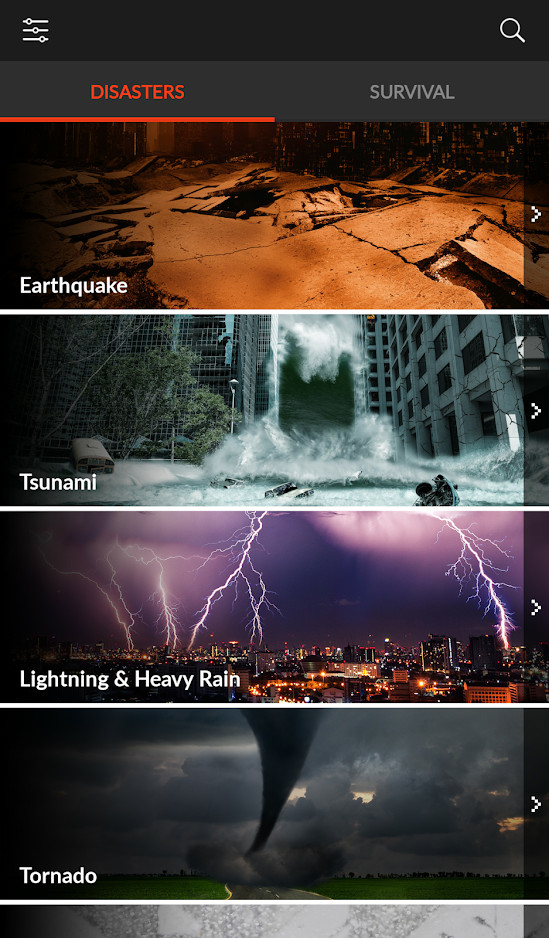
\includegraphics[height=7cm]{appImages/EPD1.jpg}
    \qquad
    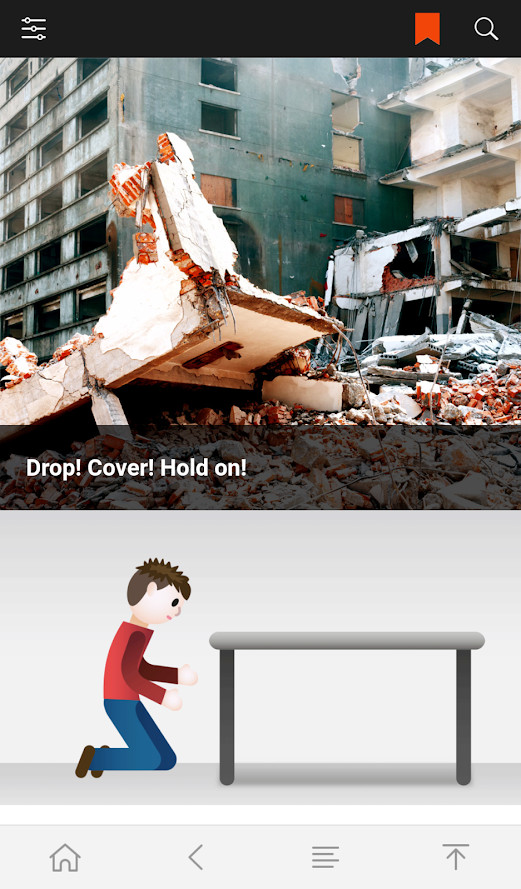
\includegraphics[height=7cm]{appImages/EPD2.jpg}
    \caption[Emergency preparedness \& Disaster Survival Guide]{Emergency preparedness \& Disaster Survival Guide is paid mobile application that cover almost all the how to survive a disastrous situation with simple  illustrations and written guides.}%
    \label{fig:app1}%
\end{figure}

   
\begin{figure}[ht!]
    \centering
    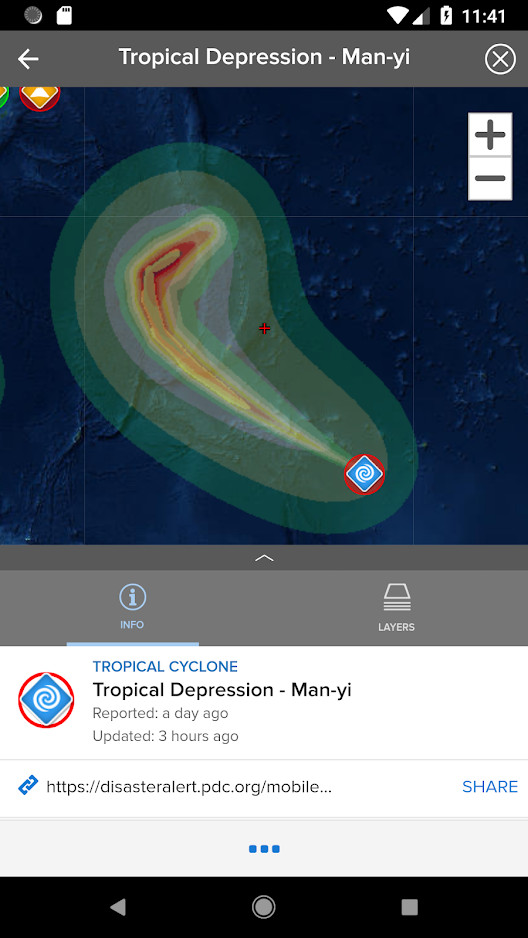
\includegraphics[height=7cm]{appImages/DA1.jpg}
    \caption[Disaster Alert\textsuperscript{\texttrademark}]{Disaster Alert is a free, mobile app that provides individuals, families, and their loved ones with the information they need to stay safe anywhere in the world. Disaster Alert offers near real-time updates about 18 different types of active hazards as they are unfolding around the globe.}
    \label{fig:app2}
\end{figure}


% \chapter{External Interface Requirements}

% \section{User Interfaces}
% $<$Describe the logical characteristics of each interface between the software 
% product and the users. This may include sample screen images, any GUI standards 
% or product family style guides that are to be followed, screen layout 
% constraints, standard buttons and functions (e.g., help) that will appear on 
% every screen, keyboard shortcuts, error message display standards, and so on.  
% Define the software components for which a user interface is needed. Details of 
% the user interface design should be documented in a separate user interface 
% specification.$>$

% \section{Hardware Interfaces}
% $<$Describe the logical and physical characteristics of each interface between 
% the software product and the hardware components of the system. This may include 
% the supported device types, the nature of the data and control interactions 
% between the software and the hardware, and communication protocols to be 
% used.$>$

% \section{Software Interfaces}
% $<$Describe the connections between this product and other specific software 
% components (name and version), including databases, operating systems, tools, 
% libraries, and integrated commercial components. Identify the data items or 
% messages coming into the system and going out and describe the purpose of each.  
% Describe the services needed and the nature of communications. Refer to 
% documents that describe detailed application programming interface protocols.  
% Identify data that will be shared across software components. If the data 
% sharing mechanism must be implemented in a specific way (for example, use of a 
% global data area in a multitasking operating system), specify this as an 
% implementation constraint.$>$

% \section{Communications Interfaces}
% $<$Describe the requirements associated with any communications functions 
% required by this product, including e-mail, web browser, network server 
% communications protocols, electronic forms, and so on. Define any pertinent 
% message formatting. Identify any communication standards that will be used, such 
% as FTP or HTTP. Specify any communication security or encryption issues, data 
% transfer rates, and synchronization mechanisms.$>$


% \chapter{System Features}
% $<$This template illustrates organizing the functional requirements for the 
% product by system features, the major services provided by the product. You may 
% prefer to organize this section by use case, mode of operation, user class, 
% object class, functional hierarchy, or combinations of these, whatever makes the 
% most logical sense for your product.$>$

% \section{System Feature 1}
% $<$Don’t really say “System Feature 1.” State the feature name in just a few 
% words.$>$

% \subsection{Description and Priority}
% $<$Provide a short description of the feature and indicate whether it is of 
% High, Medium, or Low priority. You could also include specific priority 
% component ratings, such as benefit, penalty, cost, and risk (each rated on a 
% relative scale from a low of 1 to a high of 9).$>$

% \subsection{Stimulus/Response Sequences}
% $<$List the sequences of user actions and system responses that stimulate the 
% behavior defined for this feature. These will correspond to the dialog elements 
% associated with use cases.$>$
% User will tell the agent his current situation and based on the trained data agent will respond.


% \subsection{Functional Requirements}
% $<$Itemize the detailed functional requirements associated with this feature.  
% These are the software capabilities that must be present in order for the user 
% to carry out the services provided by the feature, or to execute the use case.  
% Include how the product should respond to anticipated error conditions or 
% invalid inputs. Requirements should be concise, complete, unambiguous, 
% verifiable, and necessary. Use “TBD” as a placeholder to indicate when necessary 
% information is not yet available.$>$

% $<$Each requirement should be uniquely identified with a sequence number or a 
% meaningful tag of some kind.$>$

% REQ-1:	REQ-2:

% \section{System Feature 2 (and so on)}
\chapter{Functional Requirements}
% \chapter{System Features}
% \section{Collecting medical information about users}
% Create profile from a during a sign-up process. Profile contains your name, bloodtype, any known diseases, etc...

\section{Relevium Watchful Smart Helper}
Communicate with the application through phone's built-in assistant.


\subsection{Description and priority}

\subsubsection{Intent}

To define how conversations work, we create intents in the agent that map user input to responses. In each intent, we define examples of user requests that can trigger the intent, what to extract from the request, and how to respond.

Generally, an intent represents one dialog turn within the conversation. The agent would match that input to its corresponding intent and return the response you defined within that intent. The agent's response usually prompts users for another utterance, which your agent will attempt to match to another intent, and the conversation continues.



\subsubsection{Intent Components}

\begin{itemize}
    \item Intent name: The name of the intent. The intent name is passed to your fulfillment and identifies the matched intent.

    \item Training phrases: Examples of what users can say to match a particular intent. Agent automatically expands these phrases to match similar user utterances.

    \item Action and parameters: Defines how relevant information (parameters) are extracted from user utterances. Examples of this kind of information include dates, times, names, places, and more. You can use parameters as input into other logic, such as looking up information, carrying out a task, or returning a response.

    \item Response: An utterance that's spoken or displayed back to the user.
\end{itemize}


\subsubsection{Primary Intents}

\begin{enumerate}
    \item Welcome Intent: When the Welcome Intent is matched, agent will respond with one of the pre-populated text responses from the \textbf{Responses}. Each time this intent is matched, agent returns one of the responses. For each subsequent matching, agent selects a different response until all responses have been used. then, it begins again choosing responses randomly.
    
    \item Fallback Intent: Triggers if a user's input is not matched by any of the regular intents or if it matches the training phrases.
    \item Follow-up Intent: provide a simple way to shape a conversation without having to create and manage contexts manually. These special intents are nested under their parent intent and are designed to handle preset replies from the user.
    \begin{enumerate}
        \item \textbf{Yes}: ``\textit{yes}", ``\textit{do it}", ``\textit{sure}, ``\textit{exactly}", ``\textit{confirm}", ``of \textit{course}", ``\textit{sounds good}", ``\textit{that's correct}", ``\textit{I don't mind}", ``\textit{I agree}".
        \item \textbf{No}: ``\textit{no}", ``\textit{don't do it}", ``\textit{definitely not}", ``\textit{not really"}, ``\textit{thanks but no}", ``\textit{not interested}", ``\textit{I don't think so}", ``\textit{I disagree}", ``\textit{I don't want that}".
        \item \textbf{Later}: ``\textit{later}", ``\textit{not yet}", ``\textit{ask me later}", ``\textit{not}", ``\textit{next time}", ``\textit{I said later}", ``\textit{some other time}", ``\textit{do it later}", ``\textit{not at the moment}", ``\textit{not at this time}".
        \item \textbf{Cancel}: ``\textit{cancel}", ``\textit{stop}", ``\textit{dismiss}", ``\textit{skip}", ``\textit{forget that}", ``\textit{stop it}", ``\textit{never mind}", ``\textit{do nothing}", ``\textit{just forget about it}", ``\textit{cancel that}".
        \item \textbf{More}: ``\textit{more}", ``\textit{more results}", ``\textit{anything else}", ``\textit{other results}", ``\textit{what else}", ``\textit{are there more}", ``\textit{tell me more}", ``\textit{show me more}", ``\textit{more information}".
        \item \textbf{Next}: ``\textit{next}", ``\textit{next page}", ``\textit{go forward}", ``\textit{show me next}", ``\textit{following result}", ``\textit{switch to the next}", ``\textit{go to the next page}", ``\textit{read the next results}", ``\textit{show me the next page}", ``\textit{show me the following results}".
        \item \textbf{Previous}: ``\textit{back}", ``\textit{previous}", ``\textit{go back}", ``\textit{previous page}", ``\textit{previous results}", ``\textit{return to the previous}", ``\textit{return to previous page}", ``\textit{go to the previous page}", ``\textit{go back to previous results}", ``\textit{read out the previous results}".
        \item \textbf{Repeat}: ``\textit{repeat}", ``\textit{repeat it}", ``\textit{come again}", ``\textit{do it again}", ``\textit{say it again}", ``\textit{say the same again}", ``\textit{please repeat that}", ``\textit{repeat these results}", ``\textit{could you repeat that}", ``\textit{repeat what you've just said}".
    \end{enumerate}
    
\end{enumerate}


\subsubsection{Context}

Contexts represent the current state of a user's request and allow your agent to carry information from one intent to another. You can use combinations of input and output contexts to control the conversational path the user takes through your dialog.

Contexts let agent control conversation flows by letting agent define specific states that a conversation must be in for an intent to match. Normally, Agent matches an intent if its training phrases closely resemble the user utterance. However, when you apply contexts to an intent, Agent will only consider that intent for matching if the context is active.

Contexts are very helpful in controlling order of intent matching \& creating different outcomes for intents with the same training phrases.

There are two types of context that let you activate and deactivate contexts and can control the flow of your conversation:

\begin{itemize}

\item Input contexts: When applied to an intent, an input context tells agent to match the intent only if the user utterance is a close match and if the context is active.
\item  Output contexts: When applied to an intent, an output context tells agent to activate a context if it's not already active or to maintain the context after the intent is matched.
\end{itemize}



\subsubsection{Entity}
Entities are the agent's mechanism for identifying and extracting useful data from natural language inputs.

While intents allow the agent to understand the motivation behind a particular user input, entities are used to pick out specific pieces of information that the users mention. Any important data we want to get from a user's request will have a corresponding entity.

% [TODO add our entities]


\subsubsection{Event}

Events allow agent to invoke intents based on something that has happened instead of what a user communicates. Agent supports events from several platforms (like Google Assistant, Slack, and more) based on actions users take on those platforms.



\newpage
\section{Voice Recognition}




\subsection{Description and priority}
Alternatively referred to as \textbf{speech recognition, voice recognition} is a computer software program or hardware device with the ability to decode the human voice. Voice recognition is commonly used to operate a device, perform commands, or write without having to use a keyboard, mouse, or press any buttons.

Today, this is done on a computer with \textbf{ASR (automatic speech recognition)} software programs. Many ASR programs require the user to "train" the ASR program to recognize their voice so that it can more accurately convert the speech to text. For example, you could say "open Internet" and the computer would open the Internet browser.
The first ASR device was used in 1952 and recognized single digits spoken by a user (it was not computer driven).

Today, ASR programs are used in many industries, including healthcare, military (e.g., F-16 fighter jets), telecommunications, and personal computing (i.e. hands-free computing).

\subsection{Methodology}

Voice recognition software on computers requires that analog audio be converted into digital signals, known as analog-to-digital conversion. For a computer to decipher a signal, it must have a digital database, or vocabulary, of words or syllables, as well as a speedy means for comparing this data to signals. The speech patterns are stored on the hard drive and loaded into memory when the program is run. A comparator checks these stored patterns against the output of the A/D converter; an action called pattern recognition.

In practice, the size of a voice recognition program's effective vocabulary is directly related to the random access memory capacity of the computer in which it is installed. A voice recognition program runs many times faster if the entire vocabulary can be loaded into RAM, as compared with searching the hard drive for some of the matches. Processing speed is critical, as well, because it affects how fast the computer can search the RAM for matches.

\subsection{Usability}

Relevium project uses voice recognition as an alternative way to carry out the communication with the user, we use it because of sometimes the user in critical situations won’t be able to use the typing method to use the Relevium mobile app, it also enhance the communication and offer the user a variety of different possible ways to use them as input method or interaction ways with our application.

\newpage




\section{Evacuation plan}
Find shortest safe path to evacuate and override traffic rules if necessary.


\subsection{Description and priority}

Evacuations are more common than many people realize. They are most frequently the results of fires and floods. Major storms such as hurricanes cause often result in mass-scale evacuations. In addition, hundreds of times a year, transportation and industrial accidents release harmful substances, forcing many people to leave their homes and places of work.

The amount of time you have to leave will depend on the hazard. If the event is a weather condition, such as a hurricane, you might have a day or two to get ready. However, many disasters allow no time for people to gather even the most basic necessities, which is why planning ahead is essential. Plan how you will assemble your family (or employees for workplace evacuation planning) and supplies and anticipate where you will go for different situations. Choose several destinations in different directions so you have options in an emergency and know the evacuation routes to get to those destinations


\subsection{Usability}

The country also lacks effective disaster preparedness system to confront natural disasters. Timely disaster warning and evacuation guideline can save lives of the people. In addition, a tourist or a blind people may face difficulties in finding safe area or shelter place prior to the occurrence of natural disasters.

\subsection{Guidelines}
There may be conditions under which you will decide to get away or there may be situations when you are ordered to leave. Follow these guidelines for evacuation:

\begin{itemize}
    \item Plan places where your family will meet, both within and outside of your immediate neighborhood.
    \item Use the Family Emergency Plan to decide these locations before a disaster.
\item If you have a car, keep the gas tank full if an evacuation seems likely. It is also good practice to maintain at least a half filled gas tank in the event of an unexpected need to evacuate. Gas stations may be closed during emergencies and unable to pump gas during power outages.
\item Plan to take one car per family to reduce congestion and delay.
\item Become familiar with alternate routes and other means of transportation out of your area. Choose several destinations in different directions so you have options in an emergency.
\item Leave early enough to avoid being trapped by severe weather.
\item Follow recommended evacuation routes.
\item Do not take shortcuts, they may be blocked.
\item Be alert for road hazards such as washed-out roads or bridges and downed power lines.
\item Do not drive into flooded areas.
\item If you do not have a car, plan how you will leave if you have to. Make arrangements with family, friends, or your local government.
\item Take your emergency supply kit unless you have reason to believe it has been contaminated.
\item Listen to a battery-powered radio and follow local evacuation instructions.
\item Take your pets with you, but understand that only service animals may be permitted in public shelters. Plan how you will care for your pets in an emergency.
\item Call or email the out-of-state contact in your family's communication plan. Tell him or her where you are going.
\item Secure your home by closing and locking doors and windows.
\item Unplug electrical equipment such as radios, televisions and small appliances. Leave freezers and refrigerators plugged in unless there is a risk of flooding. If there is damage to your home and you are instructed to do so, shut off water, gas, and electricity before leaving.
\item Leave a note telling others when you left and where you are going.
\item Wear sturdy shoes and clothing that provides some protection such as long pants, long-sleeved shirts, and a cap.
\item Check with neighbors who may need aid.
\end{itemize}

\newpage
\section{Early alerting system}
Predict hazardous environments and alert users.

The system leverage a third-party Disaster Management Server (DMS), mobile device with our application installed on it and Connect DMS to get updates about disaster (tsunami, cyclone or flood) to get automatic notification of upcoming disaster.


\section{Direct users to shelters and highlight danger zones}
% Mark users and areas as `safe' or `in-danger'.


When our application recognizes the user in probable disaster zone then application will disseminate visual and audio disaster warning and evacuation guideline including shortest path of shelter on the map of the application. Evacuation progress is also tracked using DMS.



\section{Share location with user information}
Track your location on the map and offer assistance.


\subsection{Description and priority}
Relevium tells user when a friend is nearby, it even lets you ``wave" at them and gives you the option to send a message if they wave back. Also let you tell your friends where you are and give them directions to your location. It will also let you pick a special friend (like a family member, spouse or love interest, for example) to share your location with long-term.

\subsection{Usability}

To do so, tap the blue dot indicating where you are in the map or go to the side menu in the app and tap ``Get Started" After that, just follow the same instructions but instead tap ``Share Location," then choose any number of contacts with whom you want to share your location for a few minutes, hours, months or on an on-going basis.

Those who don’t have Relevium can share through a short link via SMS. (Of course, only share that short link with someone you trust enough not to post it to the internet or share with others you don’t know or want finding you.)


\section{Network of mobiles during the disaster (MANET)}

Stands for ``Mobile Ad-hoc Network".

Connect users in the same geographical area using a wireless mesh network (WMN).



A MANET is a type of ad-hoc network that can change locations and configure itself on the fly. Because MANETS are mobile, they use wireless connections to connect to various networks. This can be a standard Wi-Fi connection, or another medium, such as a cellular or satellite transmission.

Some MANETs are restricted to a local area of wireless devices (such as a group of laptop computers), while others may be connected to the Internet. For example, A VANET (Vehicular Ad-Hoc Network), is a type of MANET that allows vehicles to communicate with roadside equipment. While the vehicles may not have a direct Internet connection, the wireless roadside equipment may be connected to the Internet, allowing data from the vehicles to be sent over the Internet. The vehicle data may be used to measure traffic conditions or keep track of trucking fleets. Because of the dynamic nature of MANETs, they are typically not very secure, so it is important to be cautious what data is sent over a MANET.

\subsection{Description and priority}

In the infrastructure based wireless networks a node can only send a packet to a destination node only via access point (in cellular network like GSM, it is called
base station). The access point establishes a network area and
only the nodes in this area can use access point’s services.
There are some unknown events, which cause access point’s
malfunction. The nodes lose their network and they are quasi
not working.

It is the biggest infrastructure’s disadvantage.
There are also some reasons to sacrifice or not to use access
point’s services. These can be cost factor, impossibility to
install access point in short time, etc. In this case, the nodes
have to build its own network. This network is called wireless
ad hoc network.

The wireless ad hoc networks only consist of nodes
equipped with transceiver. The network are created to be
independent from an infrastructure. Therefore, the nodes must
be able to arrange their own networks. Keep in mind, that
a node can now communicate only with other nodes in
its transmission range. In the infrastructure based wireless
network, the nodes can communicate with a node, which
is located in another network area, by transmitting data to
destination access point and this access point relay the data to
the desired node.

It seems like, that the ad hoc networks are not powerful
enough. Each node has its own transmission range, if these
small transmission areas are combined, they will form a much
bigger transmission area. The nodes transmit their data with
single or multiple hopping technique. Now a suitable routing
algorithm must be implemented, so the process of transmitting
data will be more effective.

\subsection{Usability}

The usability of this feature in Relevium project will occur when the infrastructure of the cellular network or WLAN isn’t available or accessible, so we can make the users who have Relevium mobile app communicate with their mobiles using Mobile ad-hoc network (MANET) to share knowledge and current situation that’s happening at each person side, and to help society collaborate and quick help each other during disasters.




\newpage
\section{Web crawler to collect data from websites}
Monitor Twitter, Reddit and other news aggregators for any events.


\subsection{Description and priority}
A Web crawler is an Internet bot which helps in Web indexing. They crawl one page at a time through a website until all pages have been indexed. Web crawlers help in collecting information about a website and the links related to them, and also help in validating the HTML code and hyperlinks.
A Web crawler is also known as a Web spider, automatic indexer or simply crawler.

\subsection{Methodology}

The crawl started by making requests to the URLs defined in the script attributes, then call callback method to pass the response object as an argument. In the parsing callback, we loop through the response elements using a CSS Selector, yield a Statements which has specific keywords



\subsection{Usability}
Web crawlers collect information such the URL of the website, the meta tag information, the Web page content, the links in the web page and the destinations leading from those links, the web page title and any other relevant information. They keep track of the URLs which have already been downloaded to avoid downloading the same page again.

A combination of policies such as re-visit policy, selection policy, parallelization policy and politeness policy determine the behavior of the Web crawler. There are many challenges for web crawlers, namely the large and continuously evolving World Wide Web, content selection trade-offs, social obligations and dealing with adversaries.

Web crawlers are the key components of Web search engines and systems that look into web pages. Web crawlers are also used in data mining, wherein pages are analyzed for different properties like statistics, and data analytic are then performed on them.

% \section{Reporting to government and NGOs}
% Help local authorities to locate users in danger during crisis.

\chapter{Non-Functional Requirements}
% [TODO]
% \chapter{Other Nonfunctional Requirements}
Nonfunctional Requirements (NFRs) define system attributes such as security, reliability, performance, maintainability, scalability, and usability. They serve as constraints or restrictions on the design of the system across the different backlogs.

\section{Performance Requirements}
% $<$If there are performance requirements for the product under various 
% circumstances, state them here and explain their rationale, to help the 
% developers understand the intent and make suitable design choices. Specify the 
% timing relationships for real time systems. Make such requirements as specific 
% as possible. You may need to state performance requirements for individual 
% functional requirements or features.$>$
What should system response times be, as measured from any point, under what circumstances?
Are there specific peak times when the load on the system will be unusually high?

\subsection{Relevium Watchful Smart Helper}
This feature should be completed in time that ranges between \textbf{(3 - 5) seconds}


\subsection{Voice Recognition}
The response time of voice recognition should be in the range between \textbf{(2.5 - 5) seconds} in case of online, and in case of offline it should be between \textbf{(2 - 4) seconds}

\subsection{Early alerting system}
This system triggered in the online mode before the disaster happen, so any short delay in response will
be acceptable and the response time should be between \textbf{(7 - 10) seconds} and under load it 

\subsection{Network of mobiles during the disaster (MANET)}
This feature is meant to be used in offline mode and during disasters, so it should have maximum time of \textbf{10 seconds} for critical conversations between people.

% \newpage

%--------------------------Skipped
\section{Safety Requirements}
% $<$Specify those requirements that are concerned with possible loss, damage, or 
% harm that could result from the use of the product. Define any safeguards or 
% actions that must be taken, as well as actions that must be prevented. Refer to 
% any external policies or regulations that state safety issues that affect the 
% product’s design or use. Define any safety certifications that must be 
% satisfied.$>$

User agrees by using this system that under no circumstances or any theories of liability under international or civil, common or statutory law including but not limited to strict liability, negligence or other tort theories or contract, patent or copyright laws, will the system be liable for damages of any kind occurring from the use of this system or any information, goods or services obtained on this website including direct, indirect, consequential, incidental, or punitive damages (even if the system has been advised of the possibility of such damages), to the fullest extent permitted by law. Some jurisdictions do not allow the exclusion or limitation of certain damages so some of these limitations may not apply to you.




\section{Security Requirements}
% $<$Specify any requirements regarding security or privacy issues surrounding use 
% of the product or protection of the data used or created by the product. Define 
% any user identity authentication requirements. Refer to any external policies or 
% regulations containing security issues that affect the product. Define any 
% security or privacy certifications that must be satisfied.$>$
This application will have users credentials like (mobile numbers, addresses ..etc)
So it must have encrypted personal data and the chat between users should be encrypted too.
Some of the supposed algorithms to be used are : \textbf{AES-256, ARC4, RSA-2048}\\


% \hrulefill

\begin{itemize}

    \item User ID: Any user who uses the system shall have a User ID.
    \item User Identification: The system requires the user to identify himself / herself using secure credentials. The user credentials are typically some form of ``username" and a matching ``password", 

\item  Modification: Any modification (insert, delete, update) for the database shall be synchronized and done only by the administrator in the ward.
\item Administrators Rights: Administrators shall be able to view and modify all information in system.
\end{itemize}

Other ``external" factors which can be used alongside the user’s identification to securely reset a password may be voice recognition, fingerprints, or smart-cards. If the person requesting the reset can show they have two or more specific elements – such as knowledge, a possession, or something inherent to the user and only the user – that only the account holder should have, then the password reset mechanism can be triggered.

\section{Software Quality Attributes}
% $<$Specify any additional quality characteristics for the product that will be 
% important to either the customers or the developers. Some to consider are: 
% adaptability, availability, correctness, flexibility, interoperability, 
% maintainability, portability, reliability, reusability, robustness, testability, 
% and usability. Write these to be specific, quantitative, and verifiable when 
% possible. At the least, clarify the relative preferences for various attributes, 
% such as ease of use over ease of learning.$>$
This mobile app should guarantee availability as it will be available every time and it must maintain lowest MTBF (mean time between failure) also it must meet correctness because any misinformation could lead to dangerous situation for the user, it should be flexible to be used easily in hard times, also it should offer the testers an instructions about how the application should be tested and what is the correct input and output, it also should be adaptable to any environment changes, app must meet portability condition as it used in a critical situations, the last but not least is the maintainability concern and it should be maintained at least one time per week.


% \section{Business Rules}
% $<$List any operating principles about the product, such as which individuals or 
% roles can perform which functions under specific circumstances. These are not 
% functional requirements in themselves, but they may imply certain functional 
% requirements to enforce the rules.$>$


% \chapter{Other Requirements}
% $<$Define any other requirements not covered elsewhere in the SRS. This might 
% include database requirements, internationalization requirements, legal 
% requirements, reuse objectives for the project, and so on. Add any new sections 
% that are pertinent to the project.$>$

\chapter{Appendix A: Analysis Models}
%see https://en.wikibooks.org/wiki/LaTeX/Glossary
% $<$Define all the terms necessary to properly interpret the SRS, including 
% acronyms and abbreviations. You may wish to build a separate glossary that spans 
% multiple projects or the entire organization, and just include terms specific to 
% a single project in each SRS.$>$

% \begin{figure}
%     \centering
%     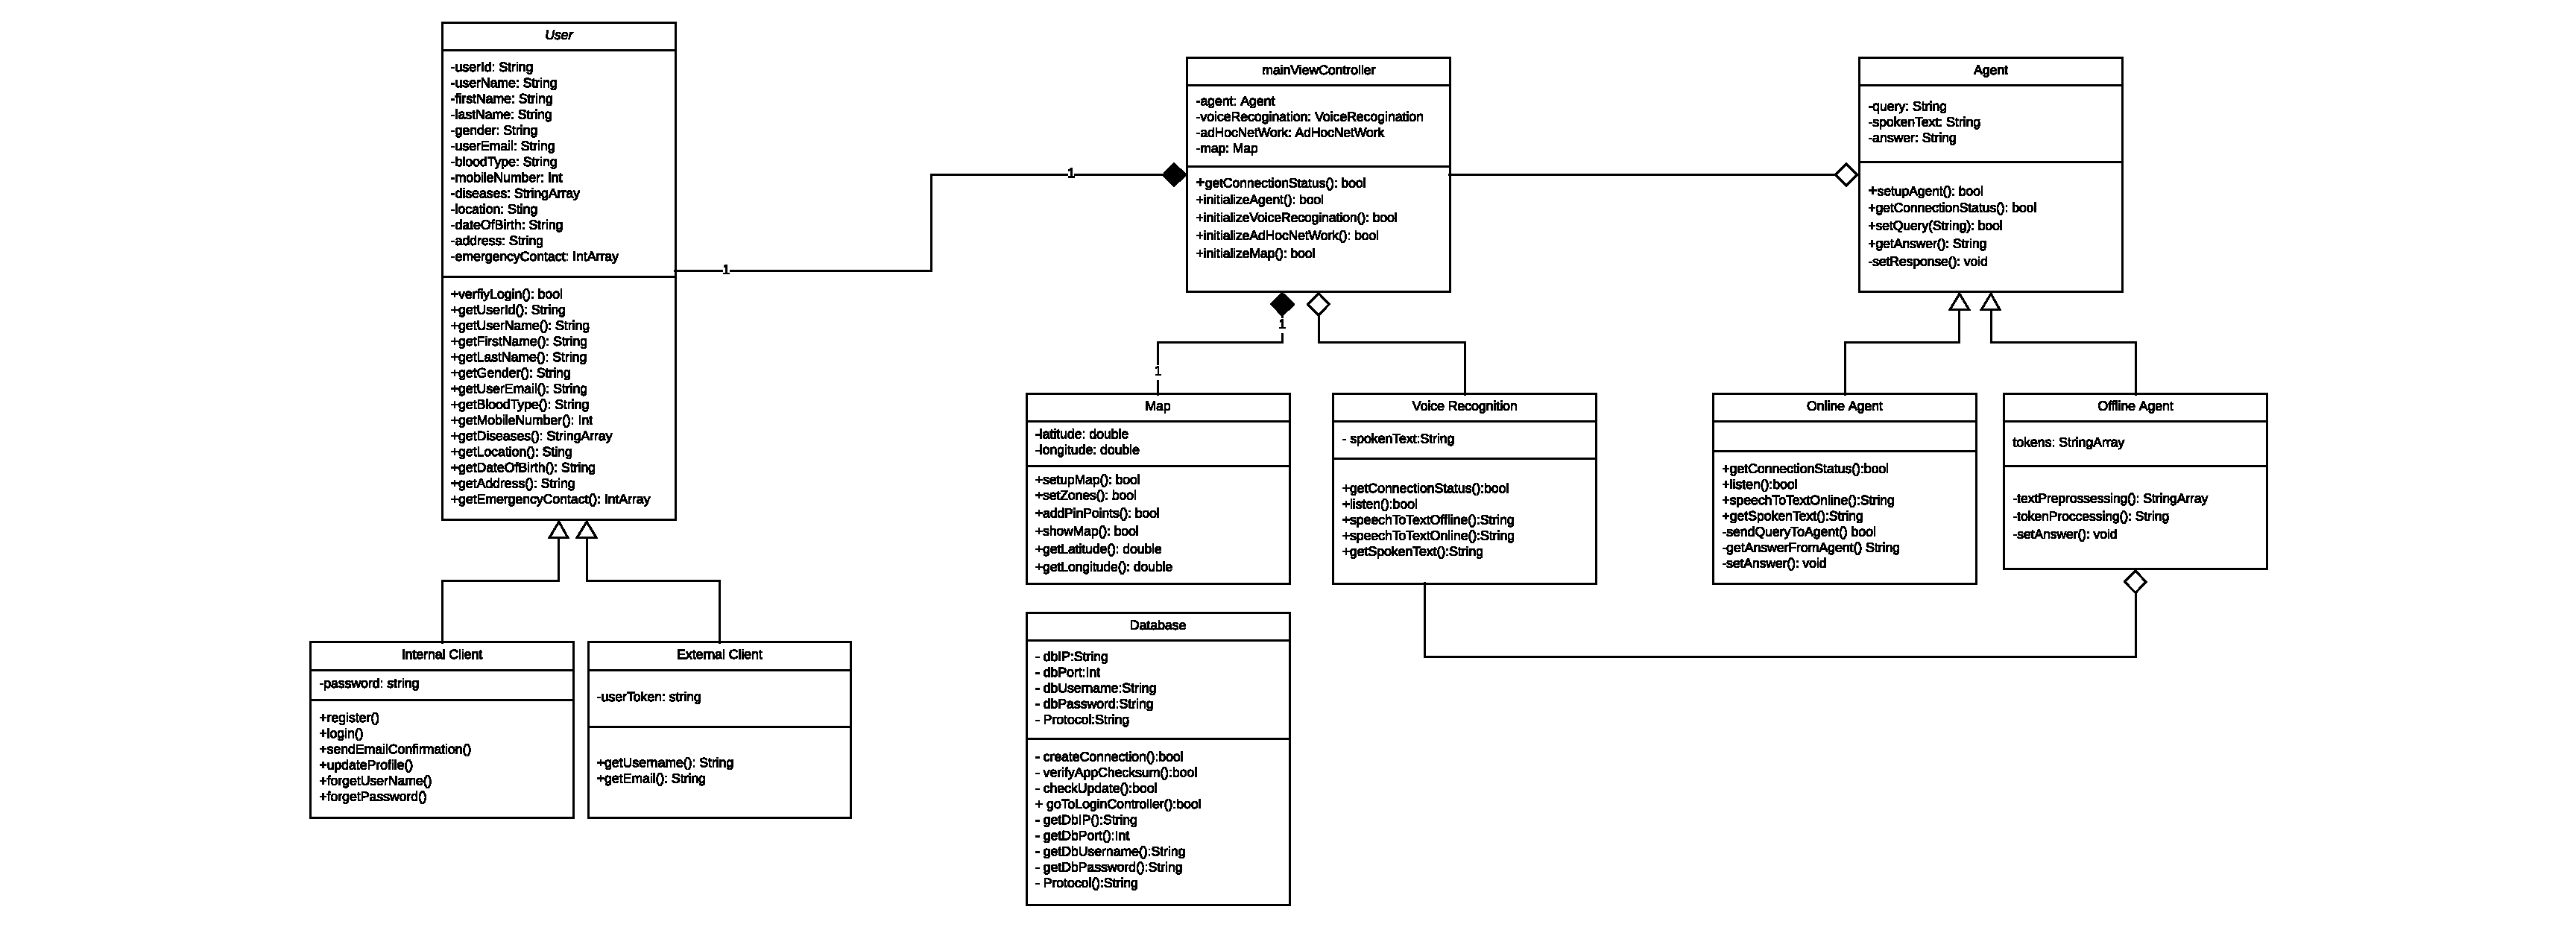
\includegraphics[angle=90, height=\textheight]{imgs/Class Diagram.pdf}
%     \caption{Class Diagram}
%     \label{fig:my_label}
% \end{figure}


    
\clearpage


\begin{figure}[ht!]
    \centering
    % \includesvg[width=0.95\textwidth]{img2/ClassD-Torky.svg}
    % 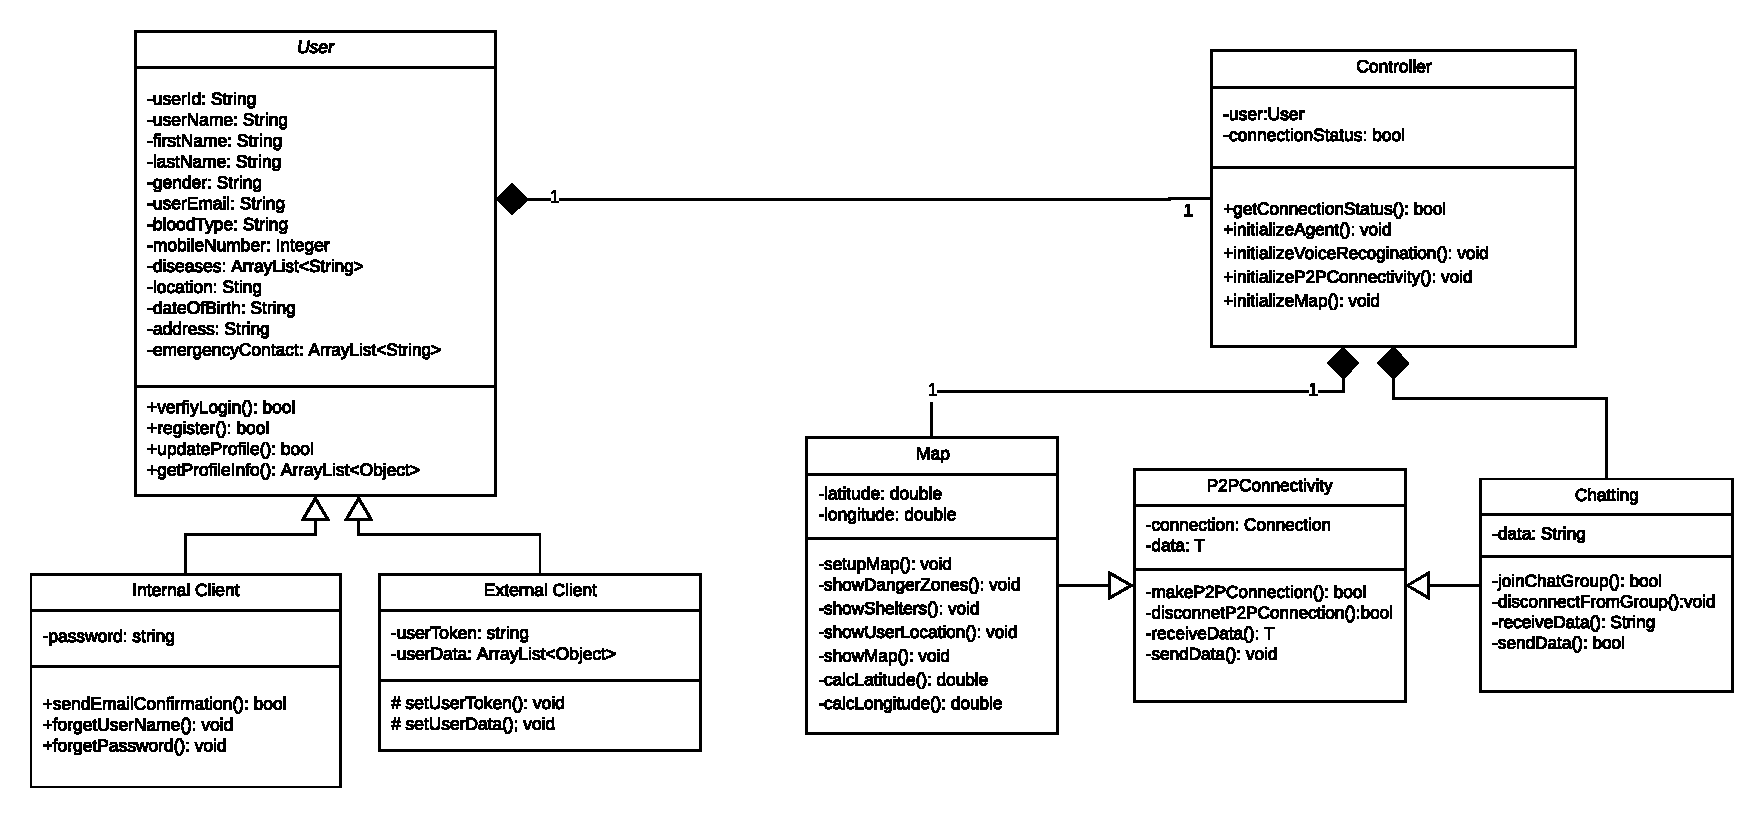
\includegraphics[angle=90, height=.92\textheight]{img2/ClassD-Torky.pdf}
    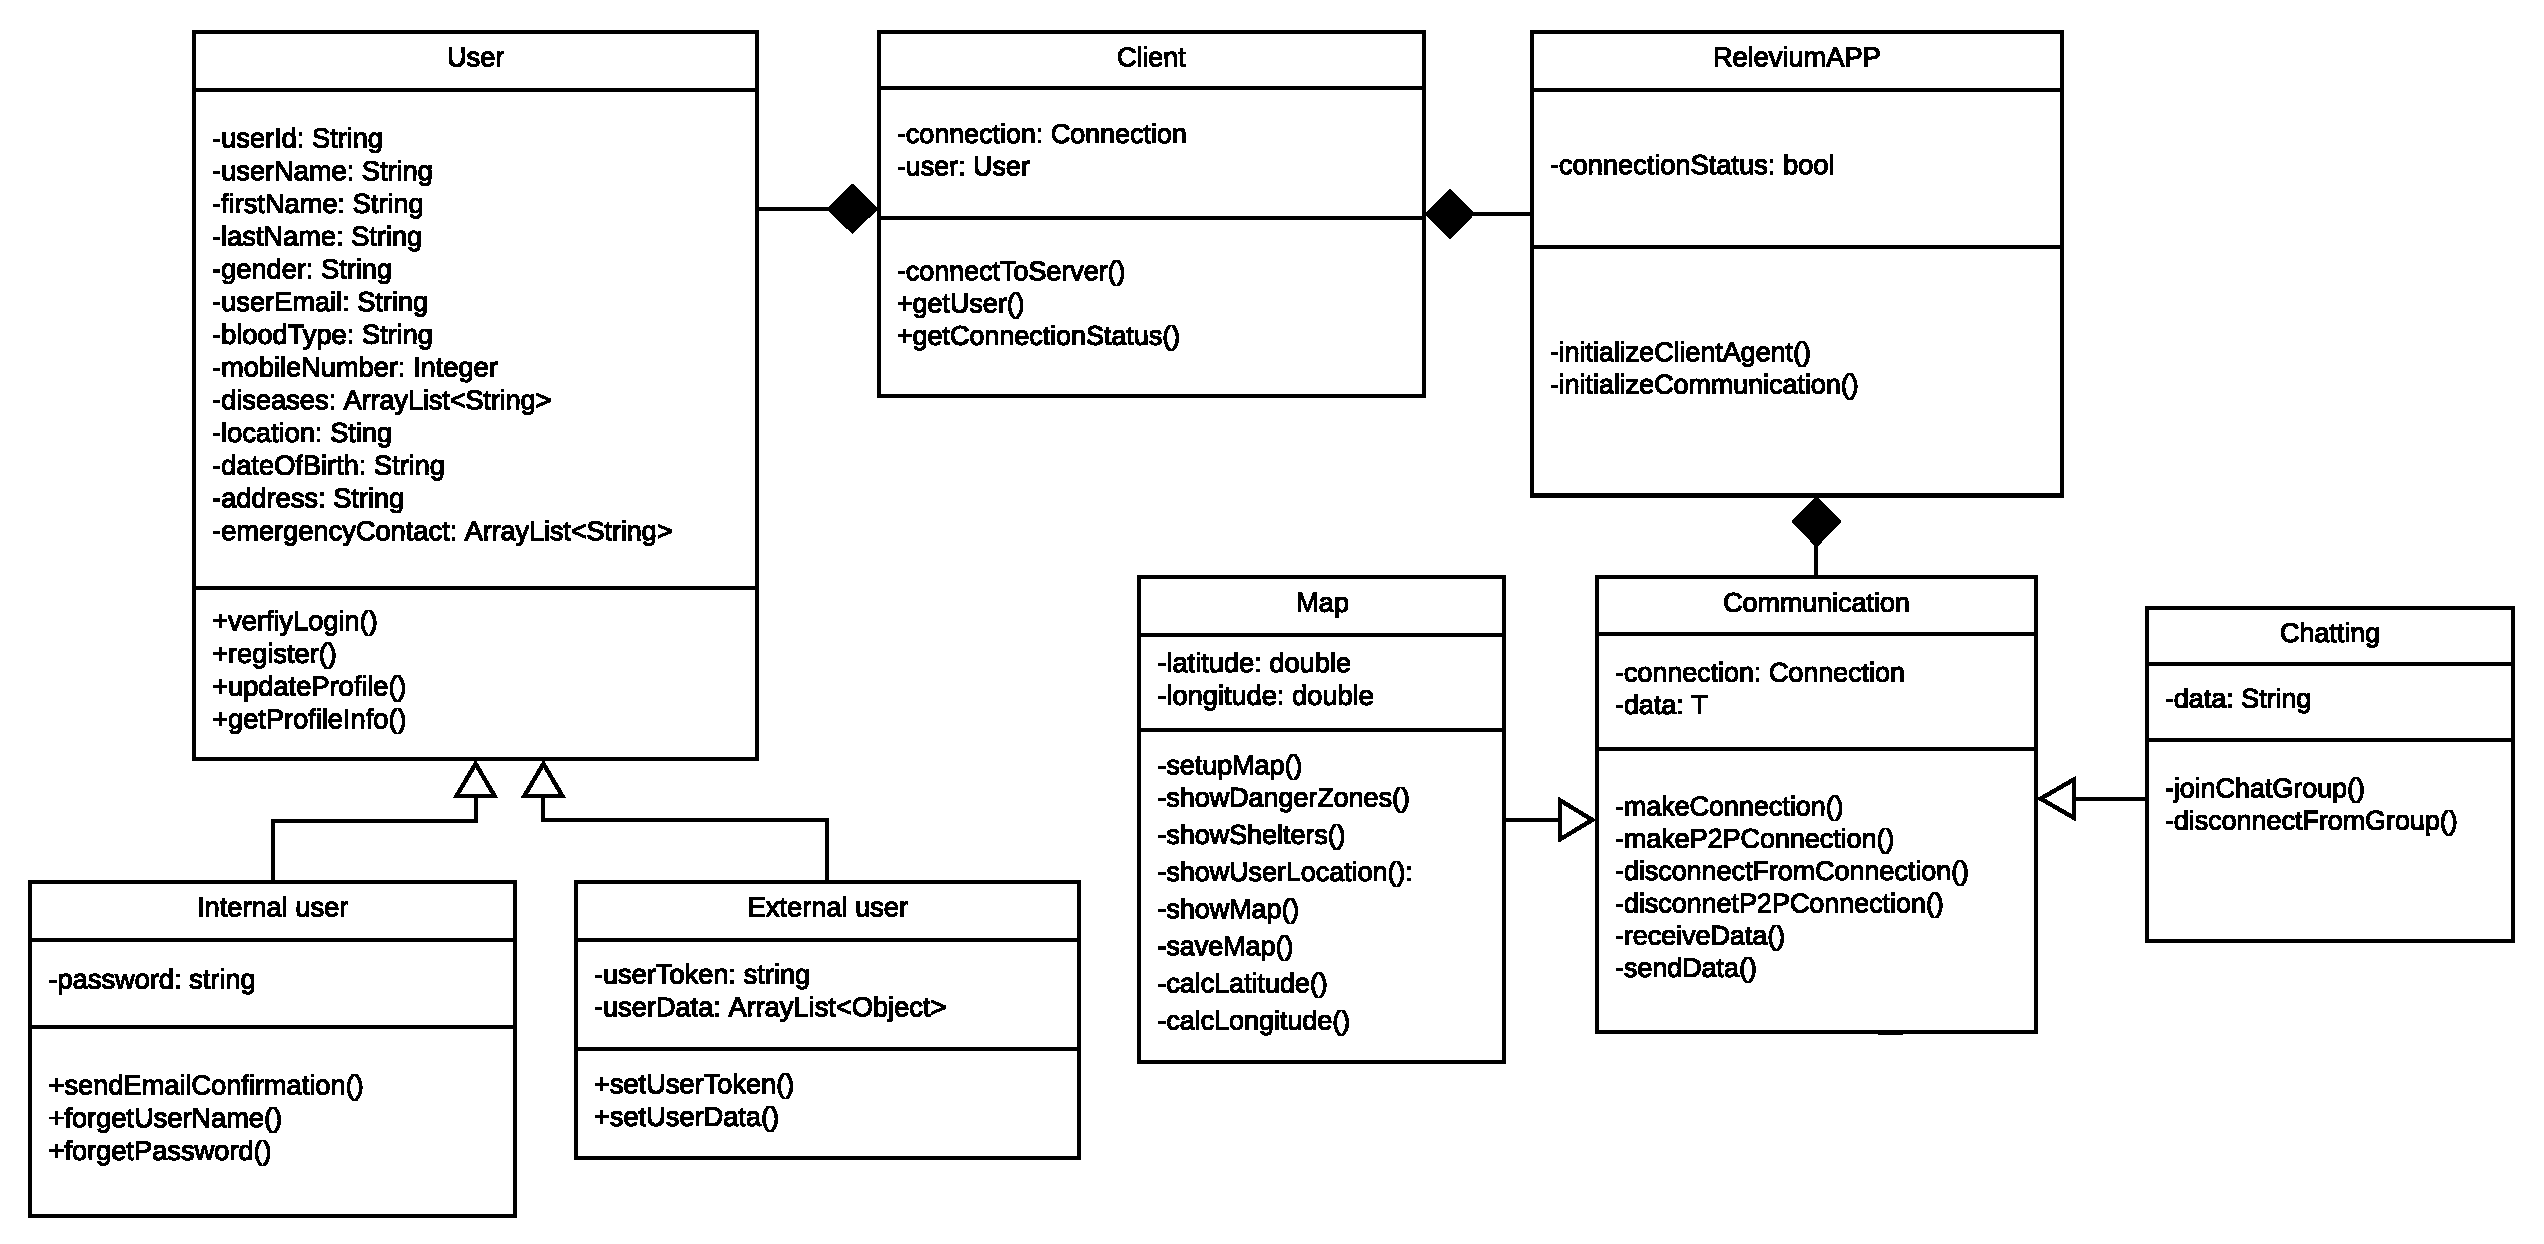
\includegraphics[angle=90, height=.92\textheight]{img3/ClassDiagram1.pdf}
    \caption{Class Diagram - Client Domain Logic}
    \label{fig:classdig1}
\end{figure}


 %% Type description here
     \textbf{User Class:} The user class contain all the information about the user, that the app uses to populate all the fields in the profile tab. All the class variables are set on the class constructor, in contrast the user can be an \textbf{\textit{internal}} or \textbf{\textit{external}} User, both \textit{\textbf{inherit}}  the class \textbf{\textit{User}}.
\begin{itemize}


\item[$\nabla$]  \textbf{verfiyLogin()}  This method takes the user ID and password or user token and authenticate it with our servers to verify user log-in credentials, finally it returns a Boolean which it's value depends on success or failure of the log-in process.
\item[$\nabla$] \textbf{register()} This method takes the user to the registration process, which asks him/her about all the required data to fill.
\item[$\nabla$] \textbf{updateProfile()} This method is used to update any user profile info and return Boolean depends on its succeed on updating or not.
\item[$\nabla$] \textbf{getProfileInfo()} This method is used by the application to populate all the fields of the the profile tab and it return an ArrayList of all the different user variable objects.

\end{itemize}

 \textbf{Internal User Class}  The internal client class is the class responsible for all the clients who registered through our servers, it handles the user log-in process, register and credentials loss.
 
 \textbf{External User Class} The external client class is the class responsible for all the clients who sign in through external API(s) eg: (Gmail, Facebook, etc...) and get their token and save it in our servers for future log-in. The class also get the data of the user from the external API after claiming the token, finally it redirect the new users to the register process with completed fields of their claimed data from the external API. If the external client did register before, then he/she will be sent to the Home screen of Relevium application.
% end of description here
% \clearpage
%%% continue description 
% \subsection{Controller Class Definition:}


     \textbf{Controller class:} is the main Activity in the mobile app by which other activity will be called,  First of all, the Controller will check the connection status as it initialed, if there is a connection available, if so it will set \textbf{connectionStatus} to be true, else it will be false. Then \textbf{User class} will be called to allow user to login, or register, then create user object, the user object will be used to display user info on the screen, or edit them.
The \textbf{mainView} which controlled by the controller should has multiple buttons, map ``initialized" by default on sub-Activity, chat, and the Assistant, and when a user push one of these buttons, activity will populate to a new sub-activity, that handle the requested function.

\begin{itemize}
% \textbf{Methods definition:}

\item[$\nabla$] \textbf{getConnectionStatus()} used to return connection Status.
\item[$\nabla$] \textbf{initializeAgent()} used to connect to the agent and populate to new sub-activity to view the agent.
\item[$\nabla$] \textbf{initializeVoiceRecogination()} used to connect to the voice Recognition and perform the requested command.
\item[$\nabla$] \textbf{initializeP2PConnectivity()} used to populate to the P2PConnectivity activity.
\item[$\nabla$] \textbf{initialzeMap()} used to populate to the map activity.
\end{itemize}

% \subsection{Map Class Definition:}

\textbf{Map class:} is the class that handle the connection between Geo-Location API and the Mobile APP, and perform all functions related to Geo-Location API.
The class will be called by controller by default after the user log-in as a sub-activity, and it inherit P2P connectivity.

% \textbf{Methods definition:}
\begin{itemize}
\item[$\nabla$] \textbf{setupMap()} used to setup connection between the Geo-location API and set all required configuration.
\item[$\nabla$] \textbf{showDangerZones()} connect to the API to set Danger zones Layers on the Map. 
\item[$\nabla$] \textbf{showShelters()} set shelters location on the map the recommend shortest path from user location to shelters.
\item[$\nabla$] \textbf{showUserLocation()} set user location on the map
\item[$\nabla$] \textbf{showMap()} used to populate map on the screen
\item[$\nabla$] \textbf{calcLatitude()} used to  set the Latitude Attribute using the GPS.
\item[$\nabla$] \textbf{calcLongitude()} used to  set the Longitude Attribute using the GPS.
\end{itemize}

% \subsection{Chatting Class Definition:}

\textbf{Chatting Class:} is the class used to handle chatting between users online and offline, so it inherit P2PConnectivity to work in offline state, the user join a group based on his location to chat with other users in the same area to ask for help or help others users. it will operate as sup-activity when the user push the chat button on the main view.

% \textbf{Methods definition:}

\begin{itemize}
\item[$\nabla$]  \textbf{joinChatGroup()} used to connect user to a chat group based on his location.
\item[$\nabla$] \textbf{disconnectFromGroup()} used to disconnect form chat group.
\item[$\nabla$] \textbf{receiveData()} used to receive data from the chat group to print it on the user screen.
\item[$\nabla$] \textbf{sendata()} used to send data to chat group.
\end{itemize}

% \subsection{P2PConnectivity Class Definition:}

\textbf{P2PConnectivity:} is the class used to  provides an easier way to create and manage sessions between users without internet connection, only via Wi-Fi or the Bluetooth. the class is inherited by map and chatting class.

\begin{itemize}

% \textbf{Methods definition:}

\item[$\nabla$] \textbf{makeP2PConnection()} is used to establish peer to peer connection with other mobile device.
\item[$\nabla$] \textbf{disconnectP2PConnection()} is used to disconnect from established connection.
\item[$\nabla$] \textbf{receiveData()} used to receive data from other device that connected with.
\item[$\nabla$] \textbf{sendData()} used to send data to other device that  connected with.
\end{itemize}
\clearpage

\begin{figure}[ht!]
    % \centering
    % \includesvg[width=\textwidth]{img2/Class1DIV.svg}
    % \hspace{-2cm}\includesvg[scale=0.4]{img2/ClassController.svg}
    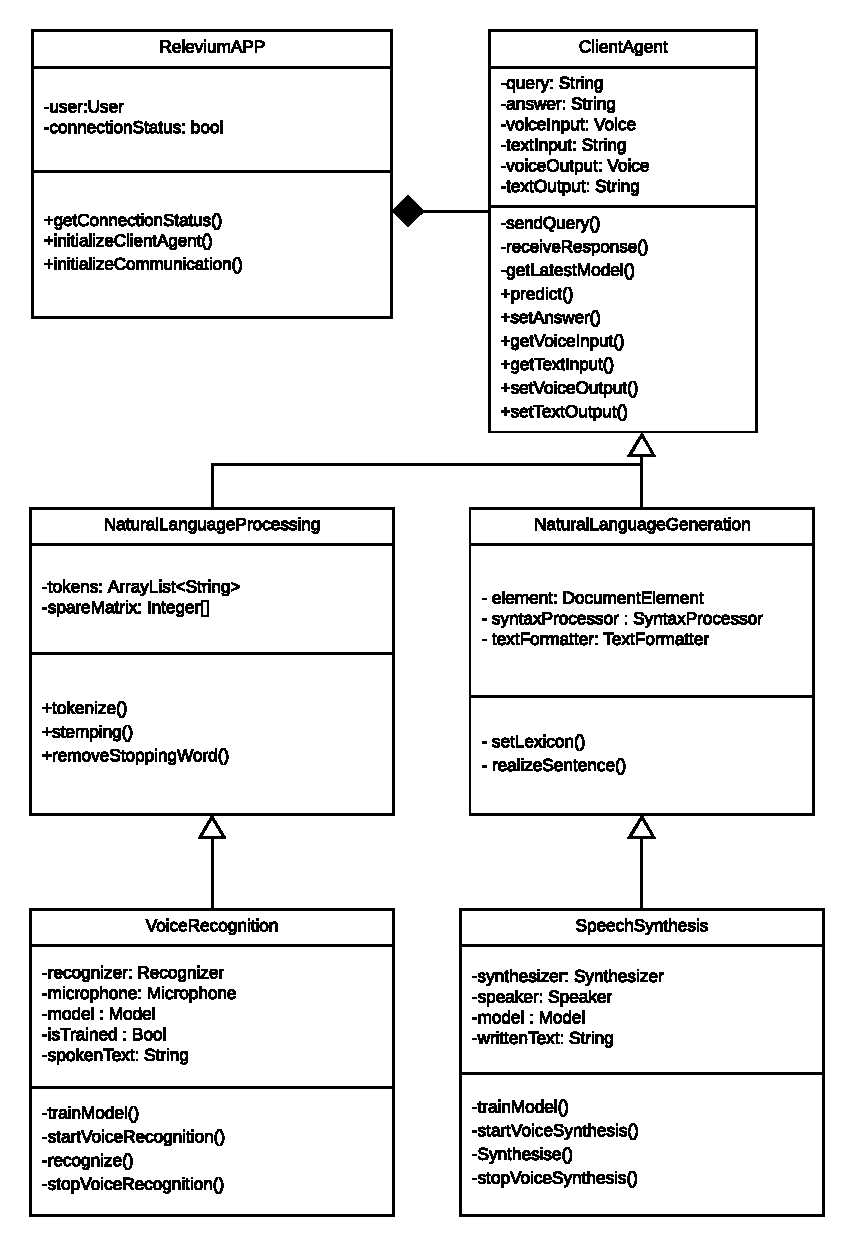
\includegraphics[height=.95\textheight]{img3/ClassDClass1DIV.pdf}
    \caption{Class Diagram - Server Domain Logic}
    \label{fig:classdiagram2}
\end{figure}

%% Type description here

% \subsection{Agent Class Definition:}
\textbf{Agent Class:} The agent class, is the class responsible for sending the user's queries to our Relevium watchful assistant servers and receive the answer from it.
\begin{itemize}
	% \textbf{Methods definition:}

	\item[$\nabla$] \textbf{sendQuery():} This method handles the network communication for sending the user query to our servers .
	\item[$\nabla$] \textbf{receiveResponse():} This method handles the network communication for receiving the appropriate answer of the user queries. 
	\item[$\nabla$] \textbf{getAnswer():} This method is used by other classes to display the received answer from the servers.
\end{itemize}


\clearpage

\begin{figure}[ht!]
    % \centering
    % \includesvg[width=\textwidth]{img2/Class1DIV.svg}
    % \hspace{-2cm}\includesvg[scale=0.4]{img2/ClassController.svg}
    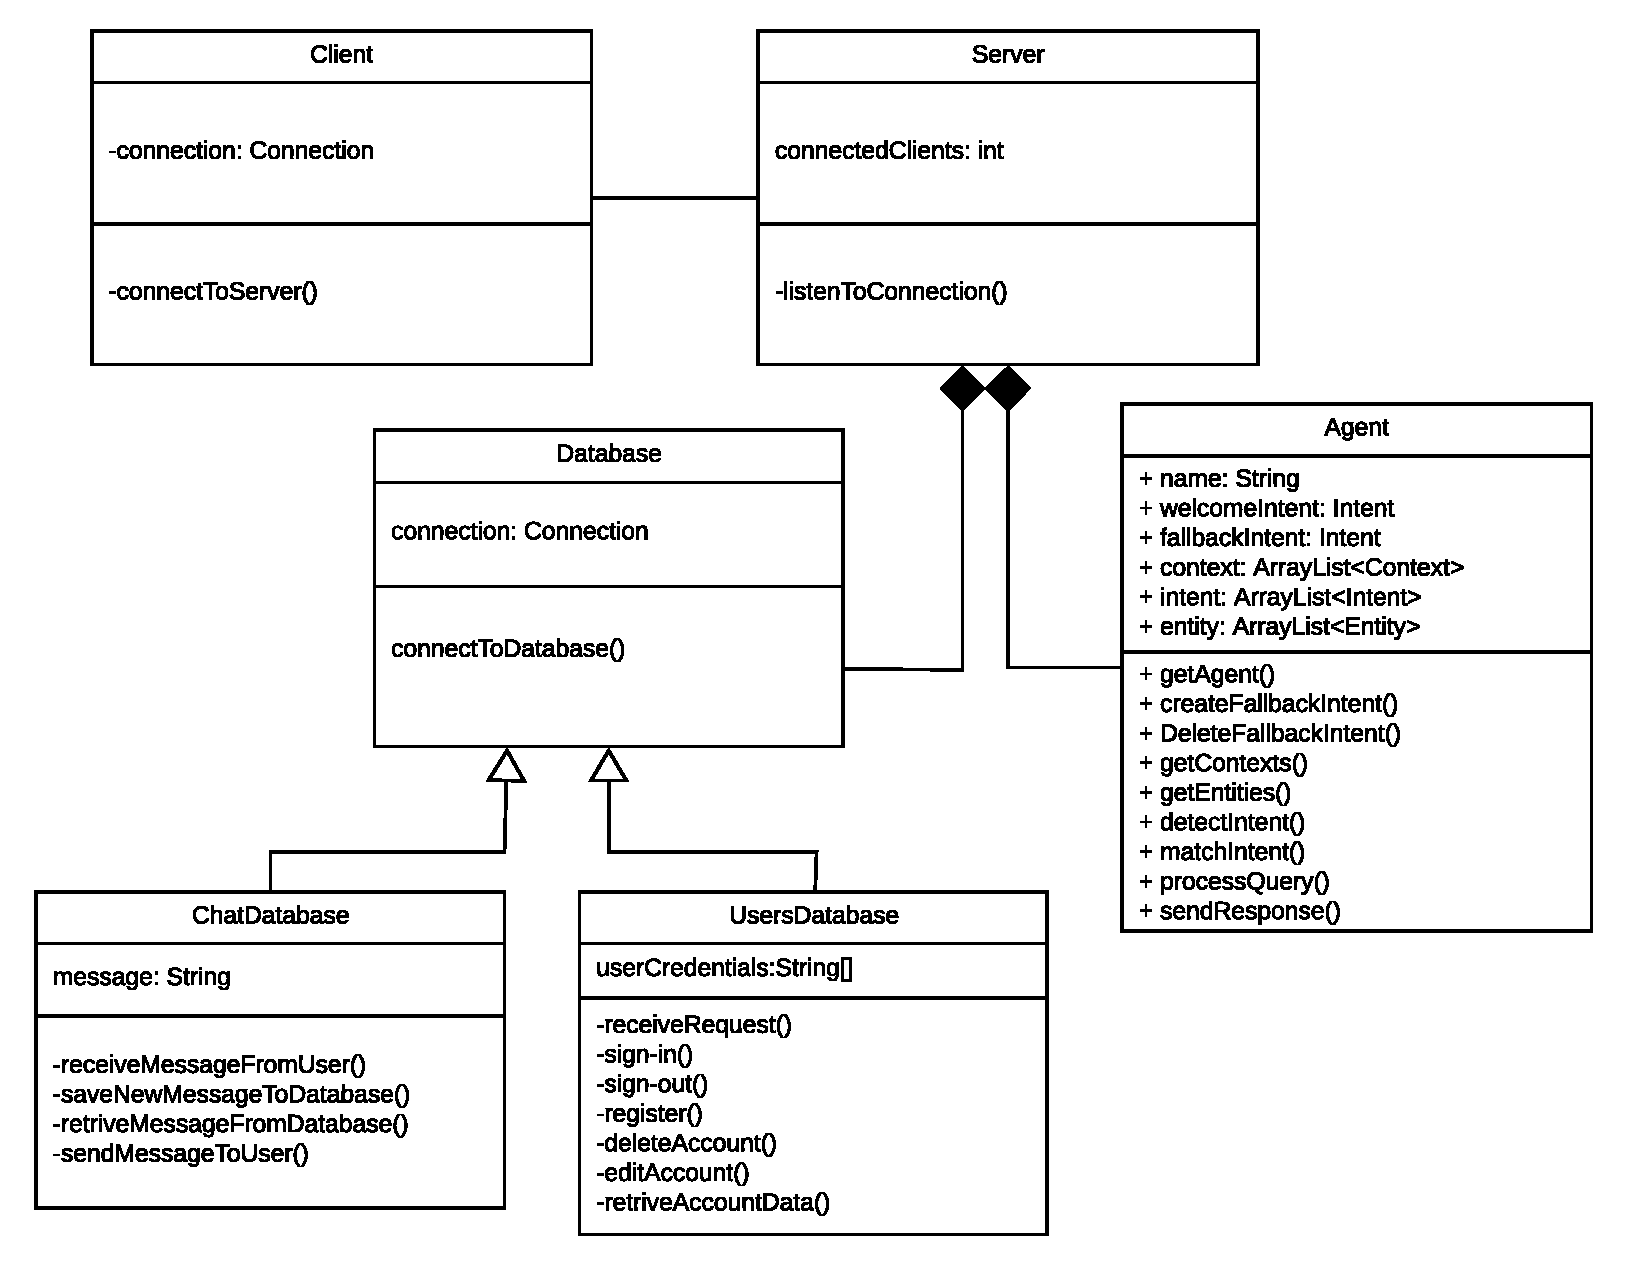
\includegraphics[angle=90, height=.95\textheight]{img3/ClassDiagramServerLogic.pdf}
    \caption{Class Diagram - Server Domain Logic (cont.)}
    \label{fig:classdiagram1}
\end{figure}



\clearpage
\begin{figure}[ht!]
    \centering
    % \includesvg[angle=90, width=1.4\textwidth]{img2/ClassDiagramAgent.svg}
    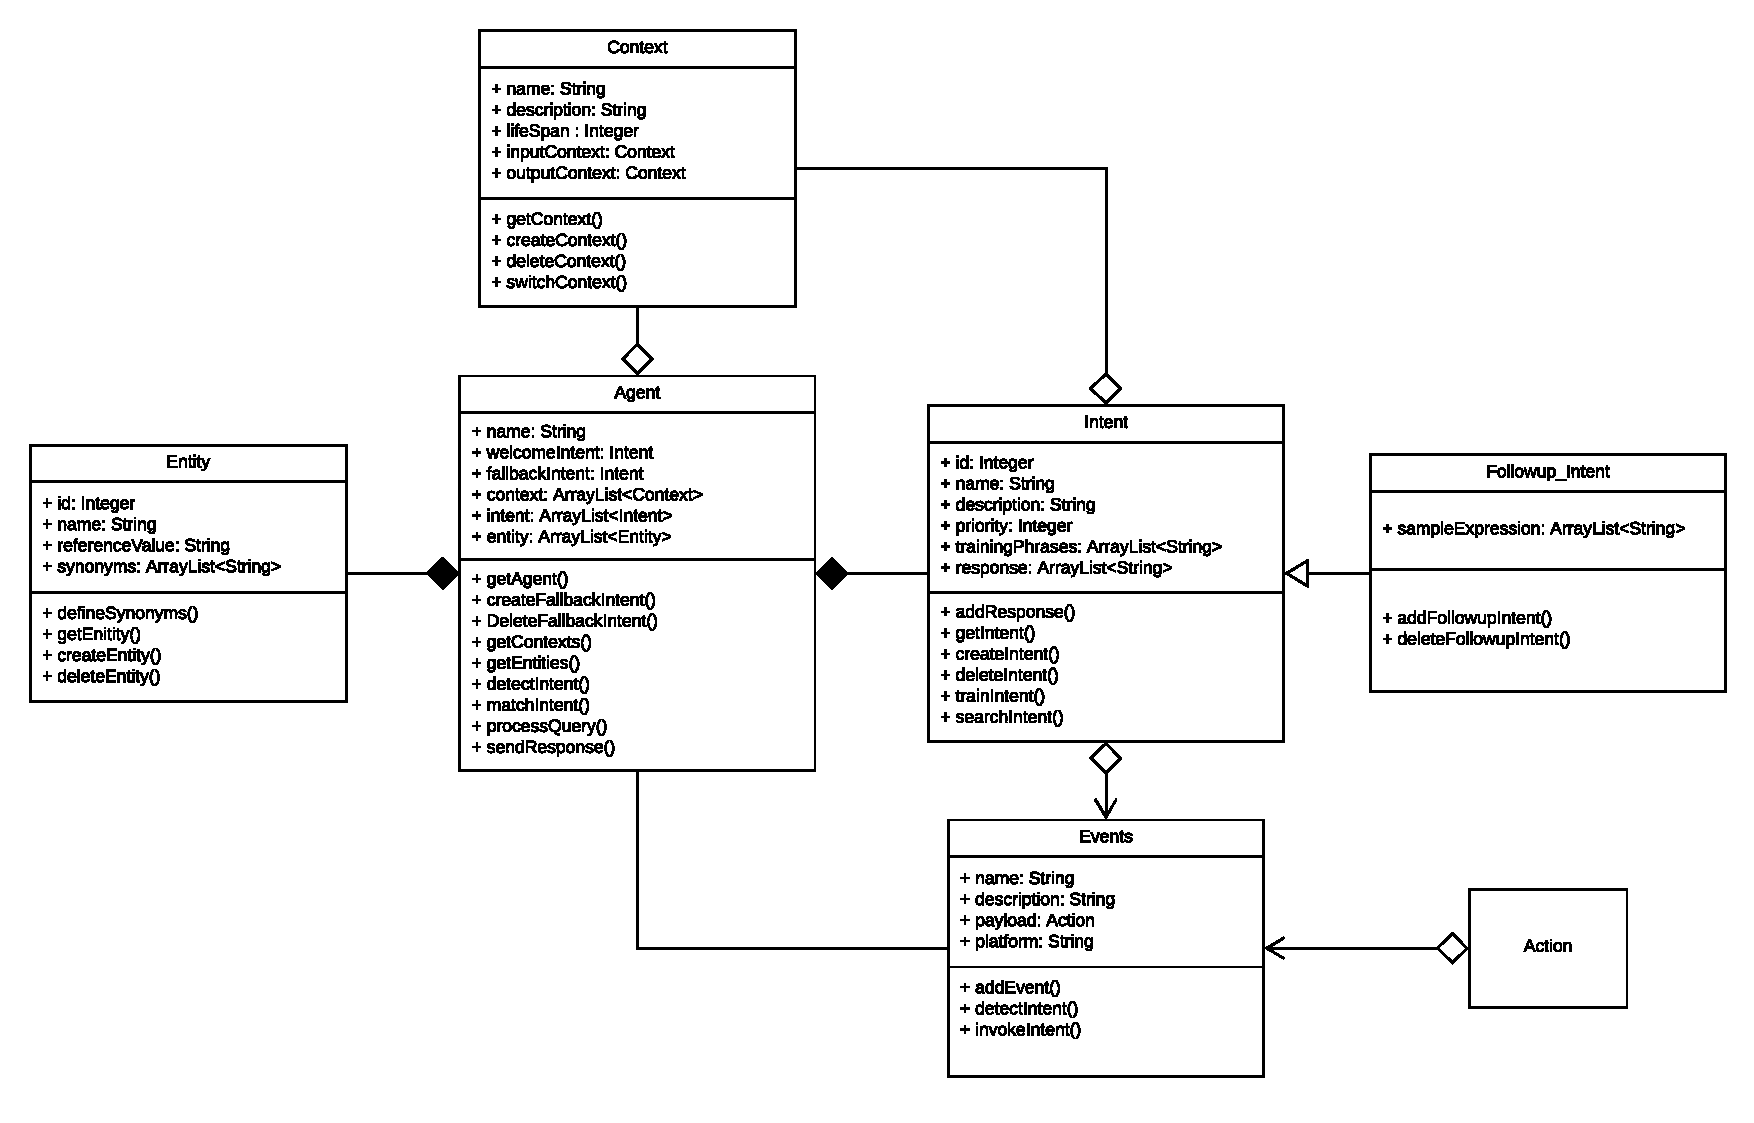
\includegraphics[angle=90, height=.94\textheight]{img2/ClassDiagramAgent.pdf}
    \caption{Class Diagram - Agent Implementation}
    \label{fig:classdiagramagent}
\end{figure}


\clearpage
\begin{figure}[ht!]
    \centering
    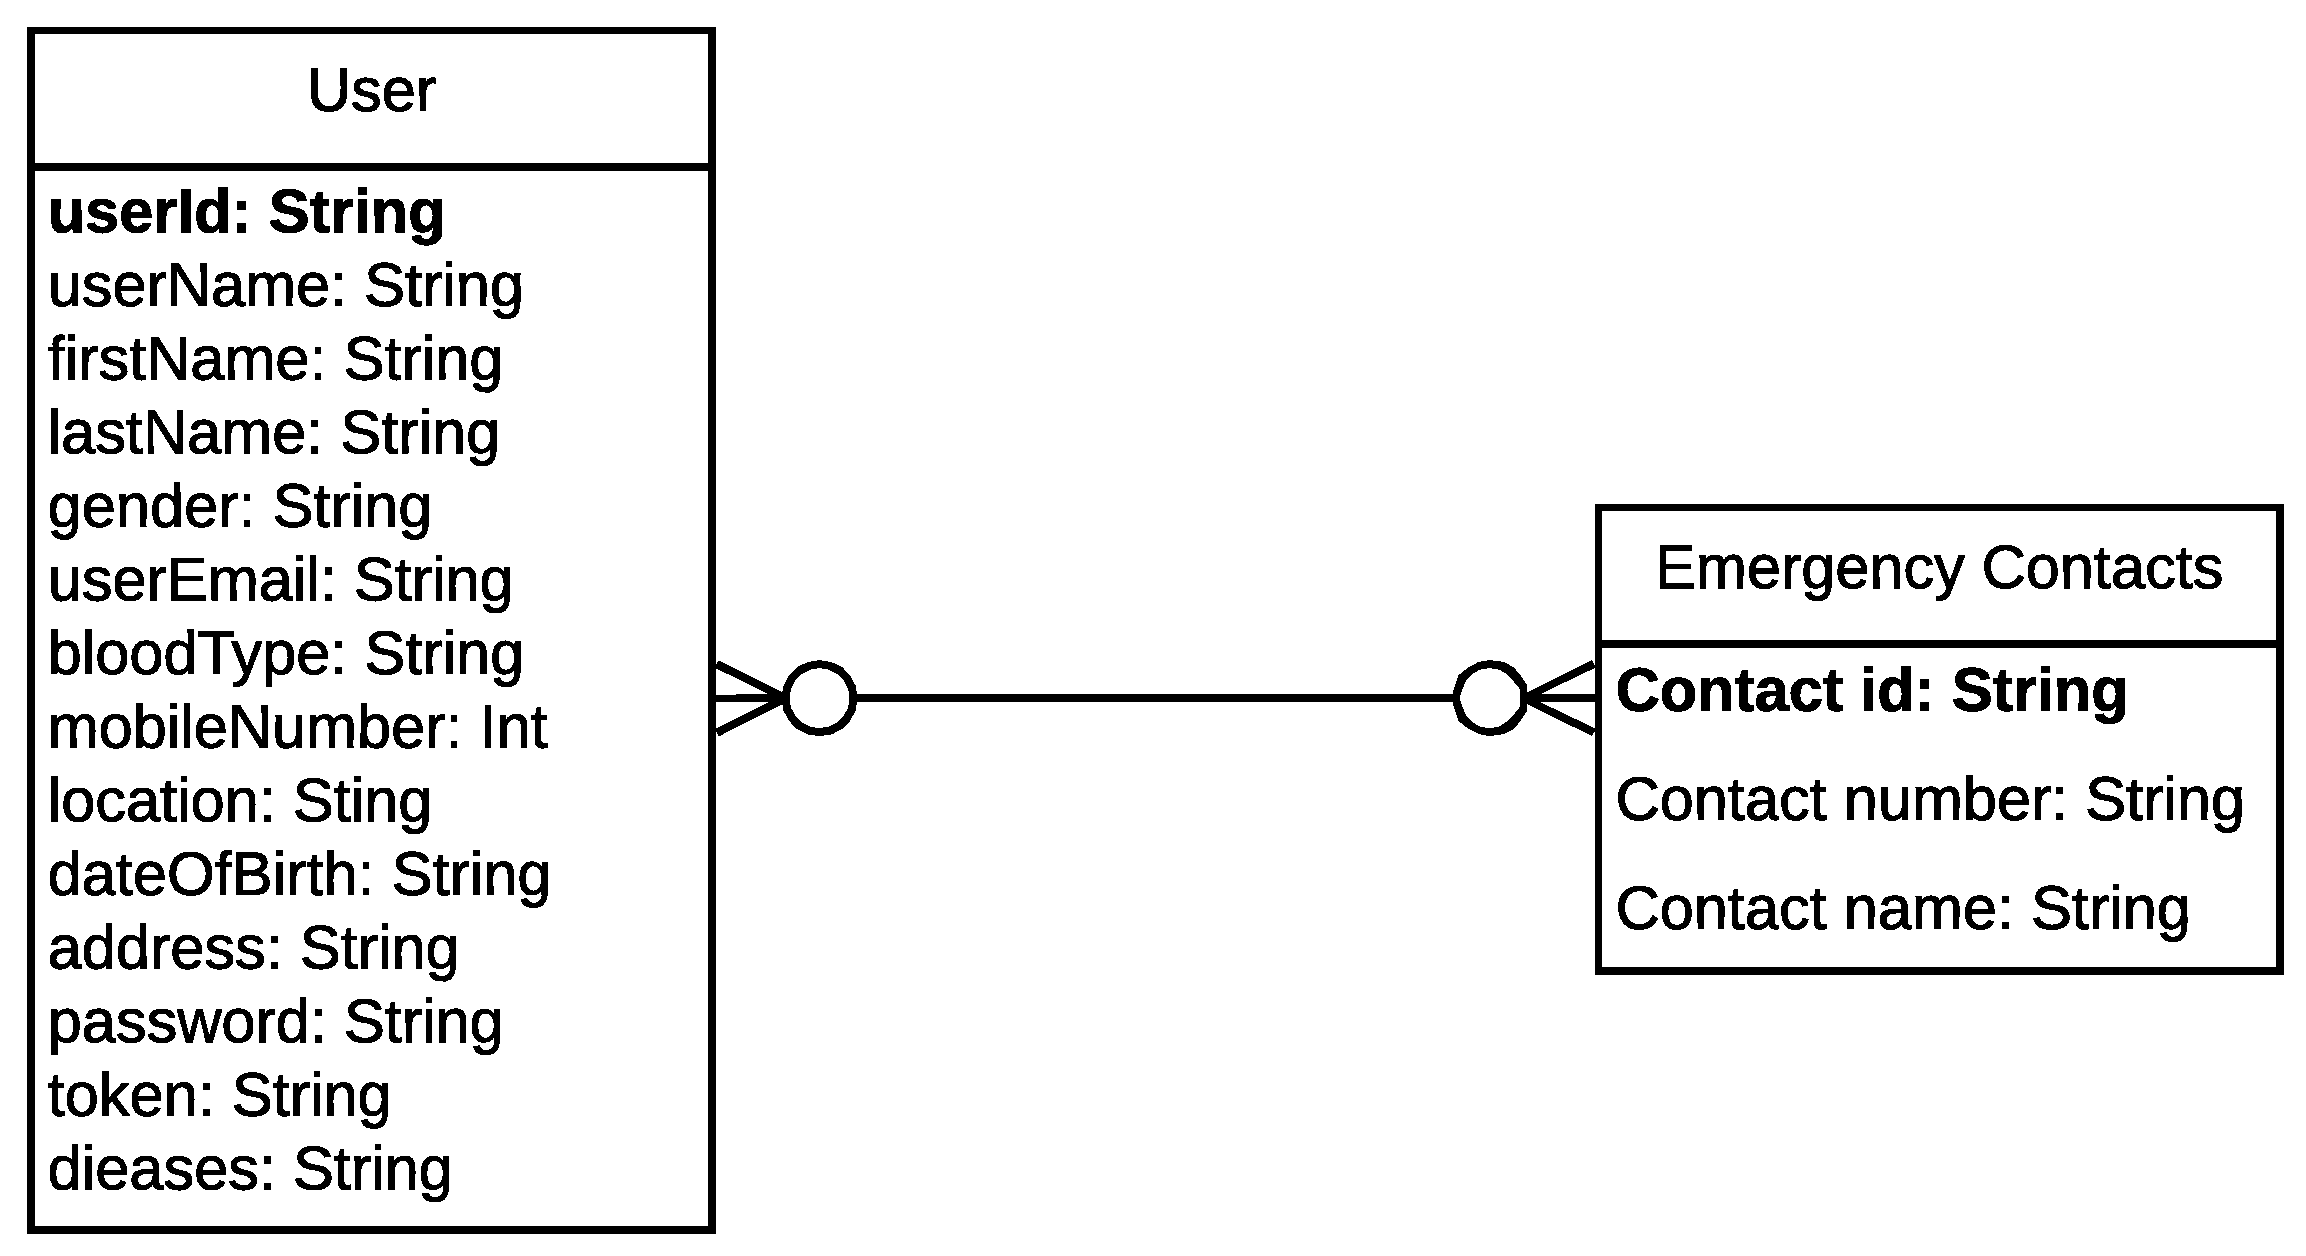
\includegraphics[angle=0, width=\textwidth]{img2/erd1.pdf}
    \caption{Entity Relationship Diagram - User}
    \label{fig:erd1}
\end{figure}



\clearpage
\begin{figure}[ht!]
    \centering
    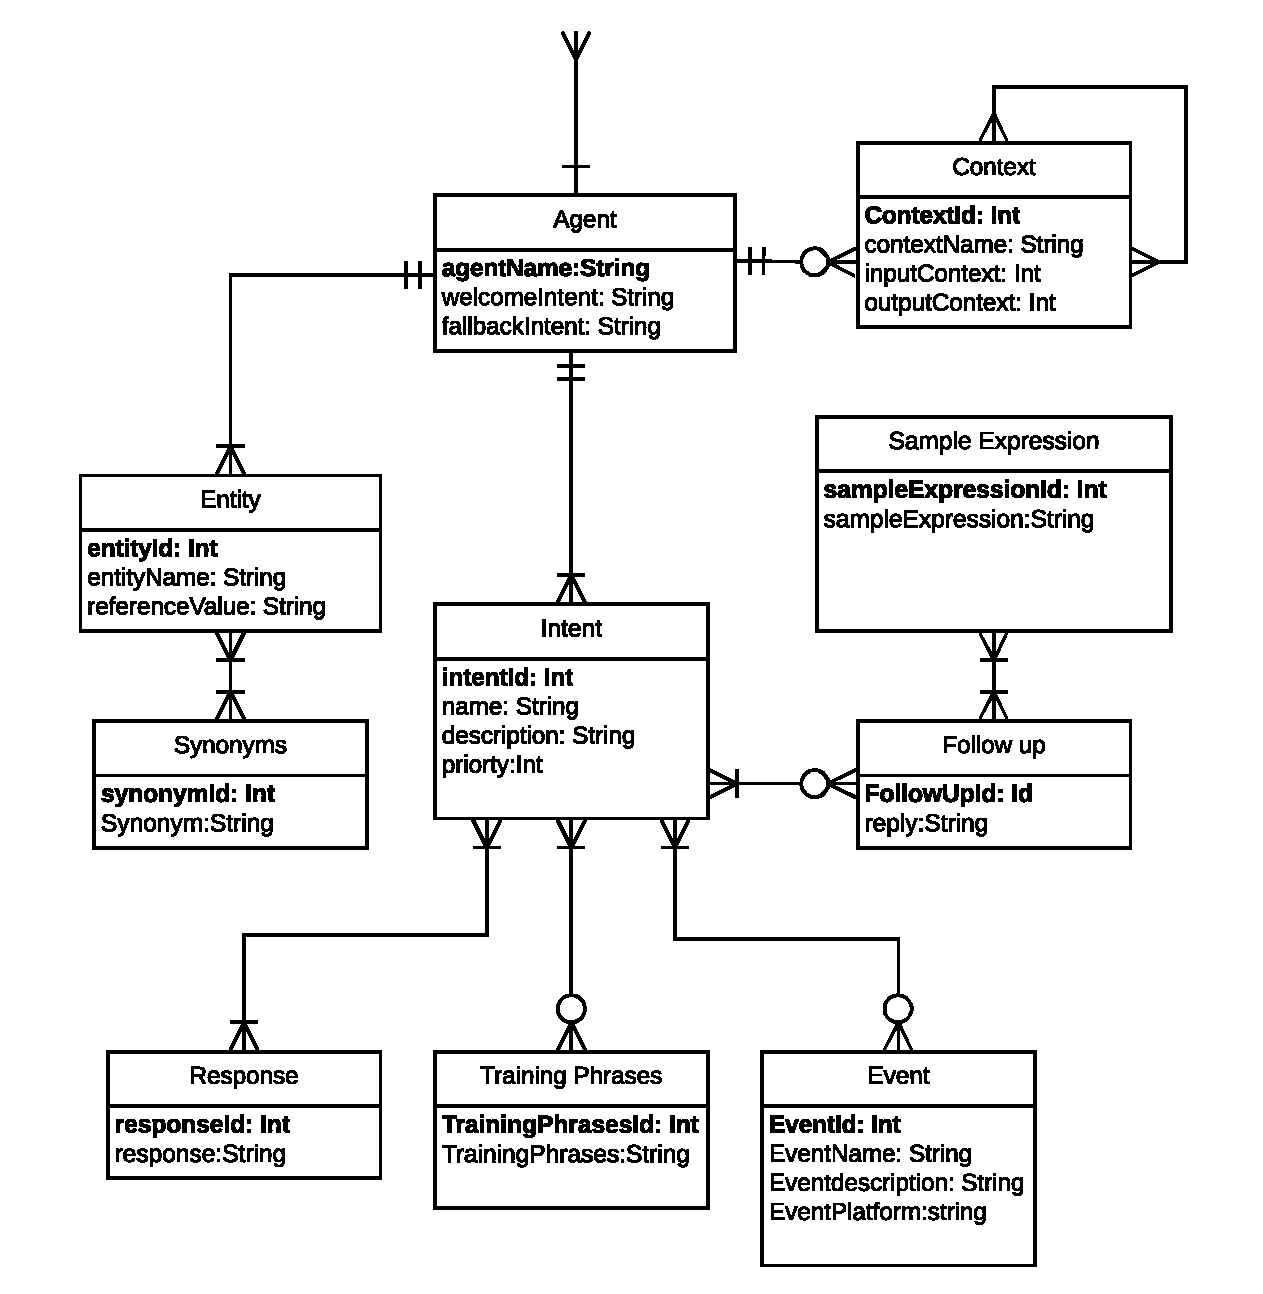
\includegraphics[angle=0, width=\textwidth]{img2/erd2.pdf}
    \caption{Entity Relationship Diagram - Agent}
    \label{fig:erd2}
\end{figure}

% \begin{figure}
%     \centering
%     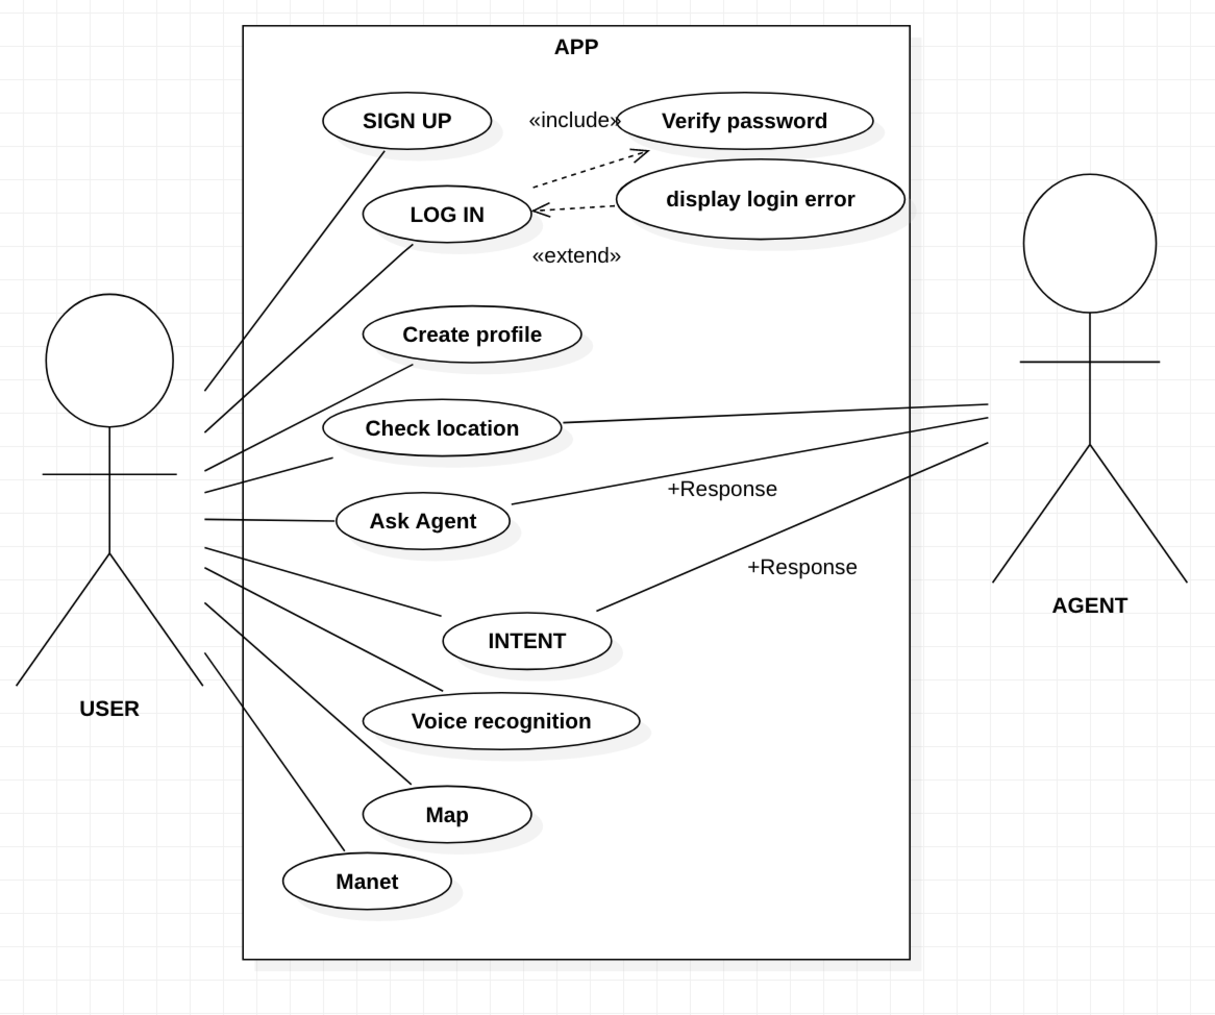
\includegraphics[angle=90, width=\textwidth]{imgs/use_case.pdf}
%     % \caption{Use Case}
%     \label{fig:my_label}
% \end{figure}

\clearpage

\begin{figure}[ht!]
    \centering
    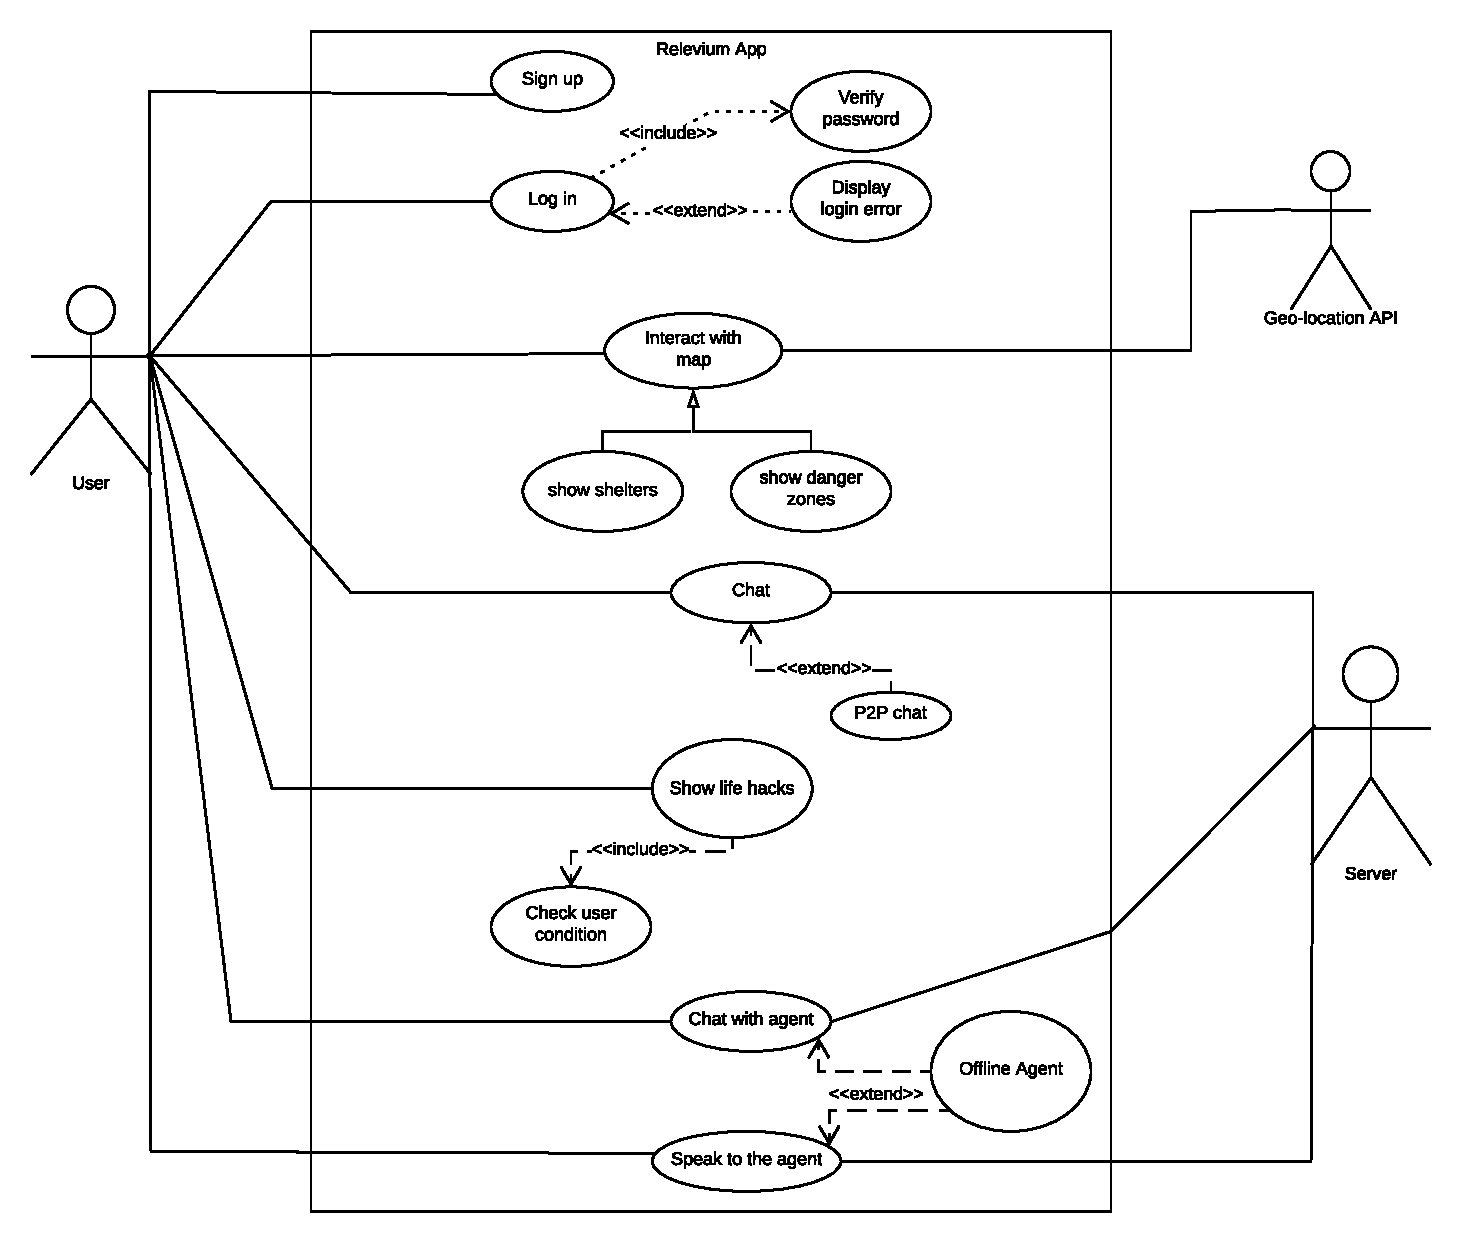
\includegraphics[width=\textwidth]{img3/UseCaseDiagram1.pdf}
    \caption{Use Case Diagram - Application Interaction}
    \label{fig:usecase1}
\end{figure}

%% Type description here
There are three actors User, Geo-Location API,Server. User: will have to sign up if he doesn't have an account and it will check for the credentials if they are correct or wrong, he also can log-in but if credentials are wrong it will display a log-in error,
he can also interact with the map to navigate danger zones and safe zones(shelters) using the information provided by Geo-Location API, during disasters each user can chat to nearby users while there are no cellular infrastructure, in addition to the user can show life hacks or some evacuation plans dependant on the current situation, user can also speak to the app.
\begin{itemize}
    \item Geo-Location API: provide the user with geo-location information.
    \item Server: Contains database and control the online chat flow with other users.
\end{itemize}


\clearpage
\begin{figure}[ht!]
    \centering
    % \includesvg[angle=90,scale=0.8]{imgs/DFDDiagram1.svg}
    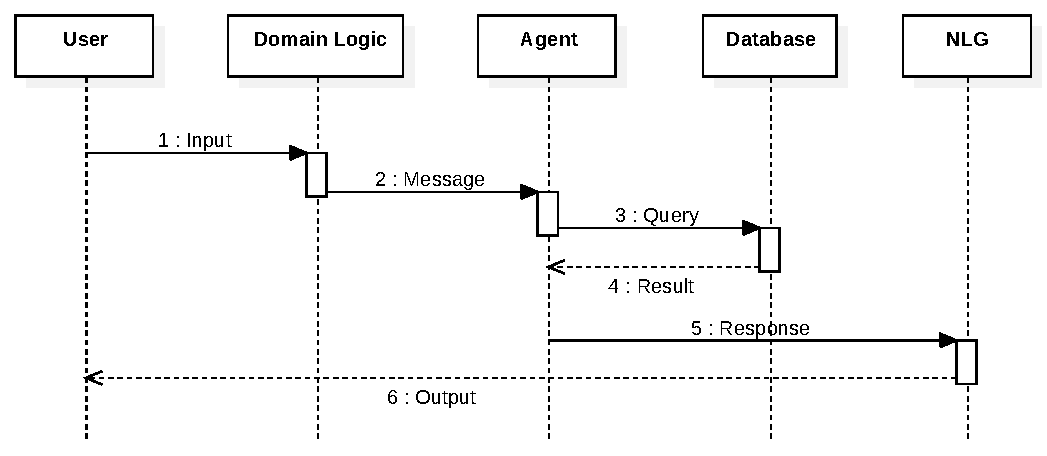
\includegraphics[angle=90, height=.95\textheight]{img3/SequenceDiagram2.pdf}
    \caption{Sequence Diagram - Utterance Route}
    \label{fig:sequence2}
\end{figure}

% \clearpage

% \begin{figure}[ht!]
%     \centering
%     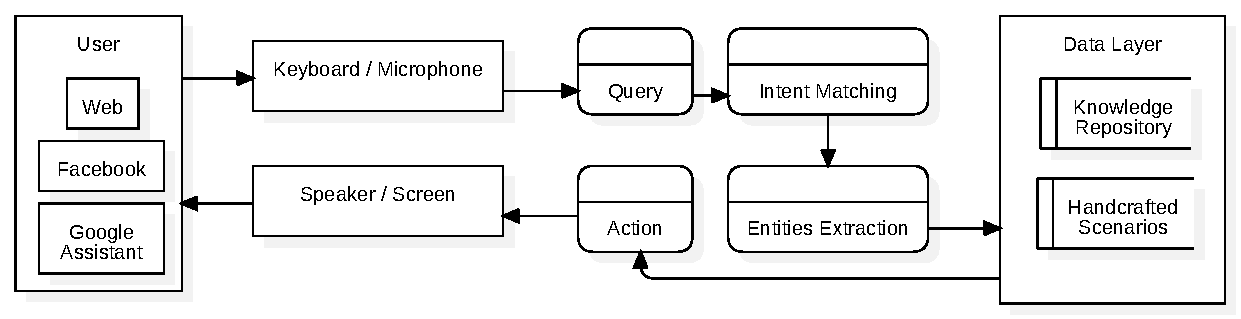
\includegraphics[angle=90, height=.95\textheight]{imgs/DFDDiagram2.pdf}
%     % \caption{Caption}
%     \label{fig:dfd2}
% \end{figure}


\clearpage

\begin{figure}[ht!]
    \centering
    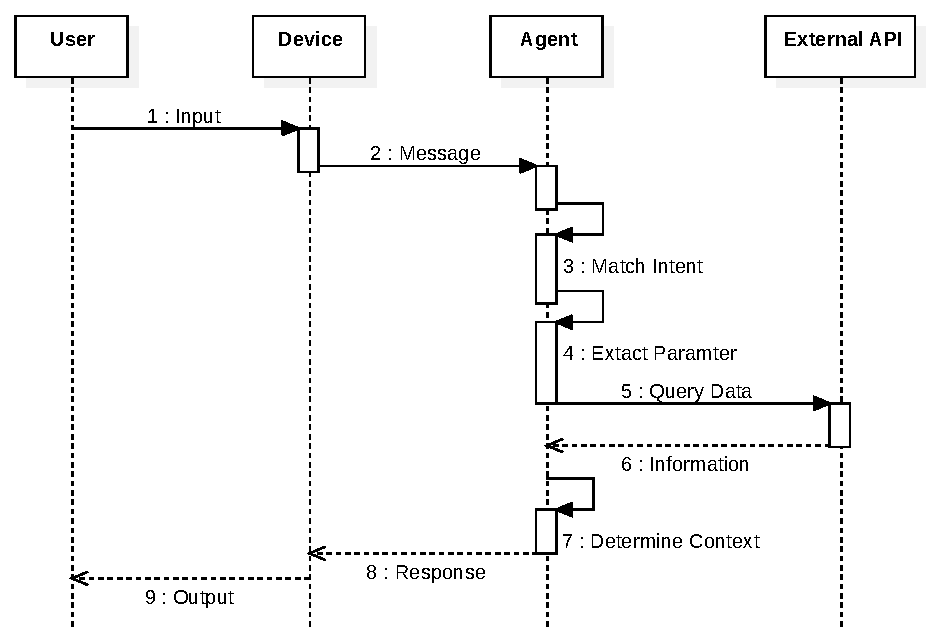
\includegraphics[angle=90, height=.95\textheight]{imgs/SequenceDiagram1.pdf}
    \caption{Sequence Diagram - Communication Process}
    \label{fig:sequencediagram1}
\end{figure}

\clearpage

\begin{figure}[ht!]
    \centering
    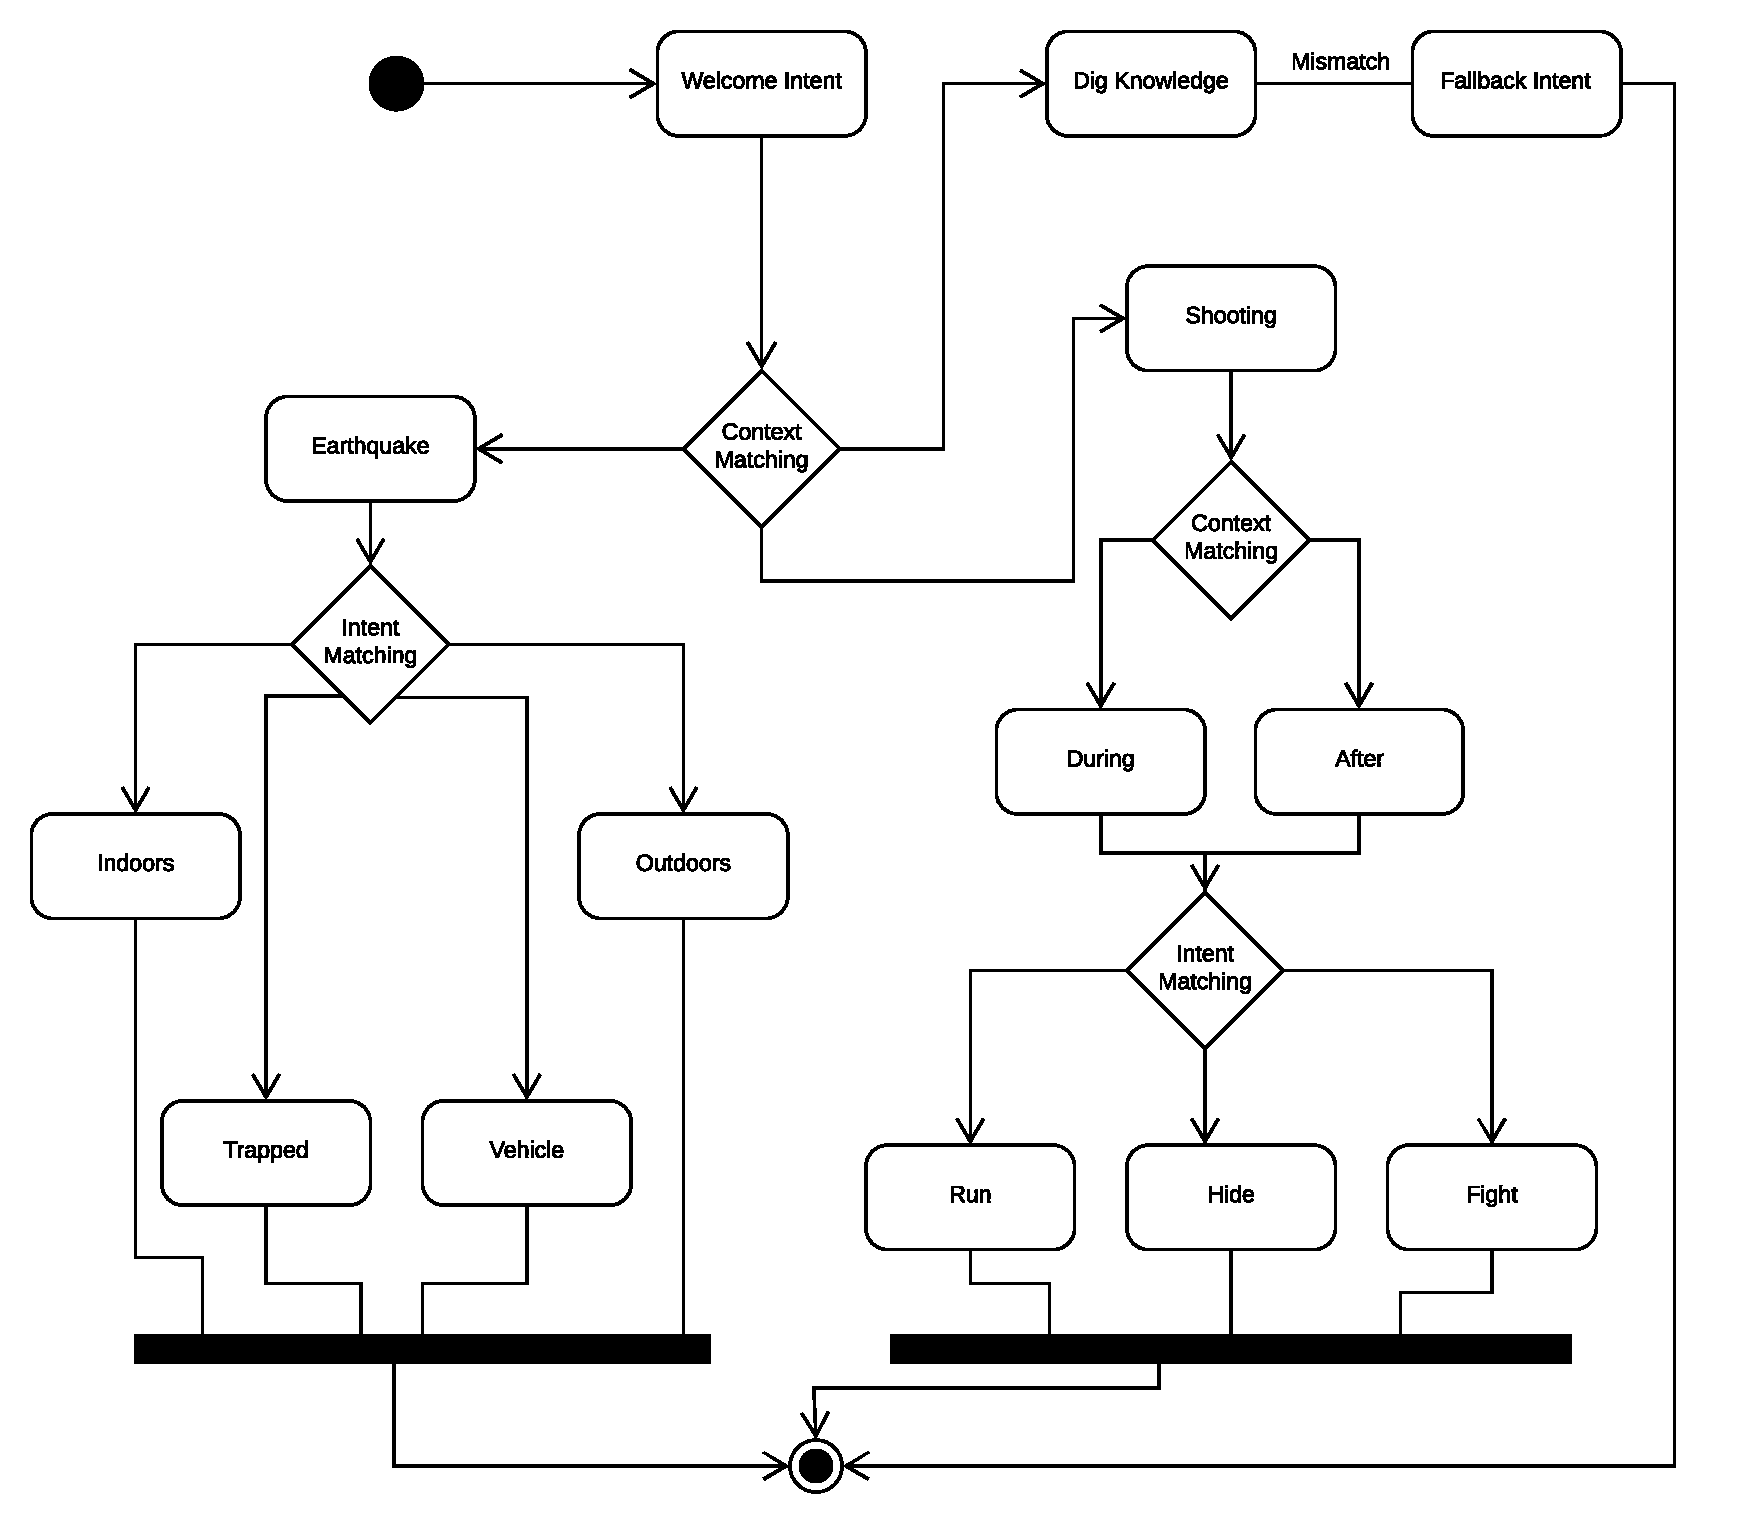
\includegraphics[angle=90, width=.95\textwidth]{img3/state1.pdf}
    \caption{State Chart Diagram - Context Matching}
    \label{fig:statechartdiagram1}
\end{figure}

\clearpage

\begin{figure}[ht!]
    \centering
    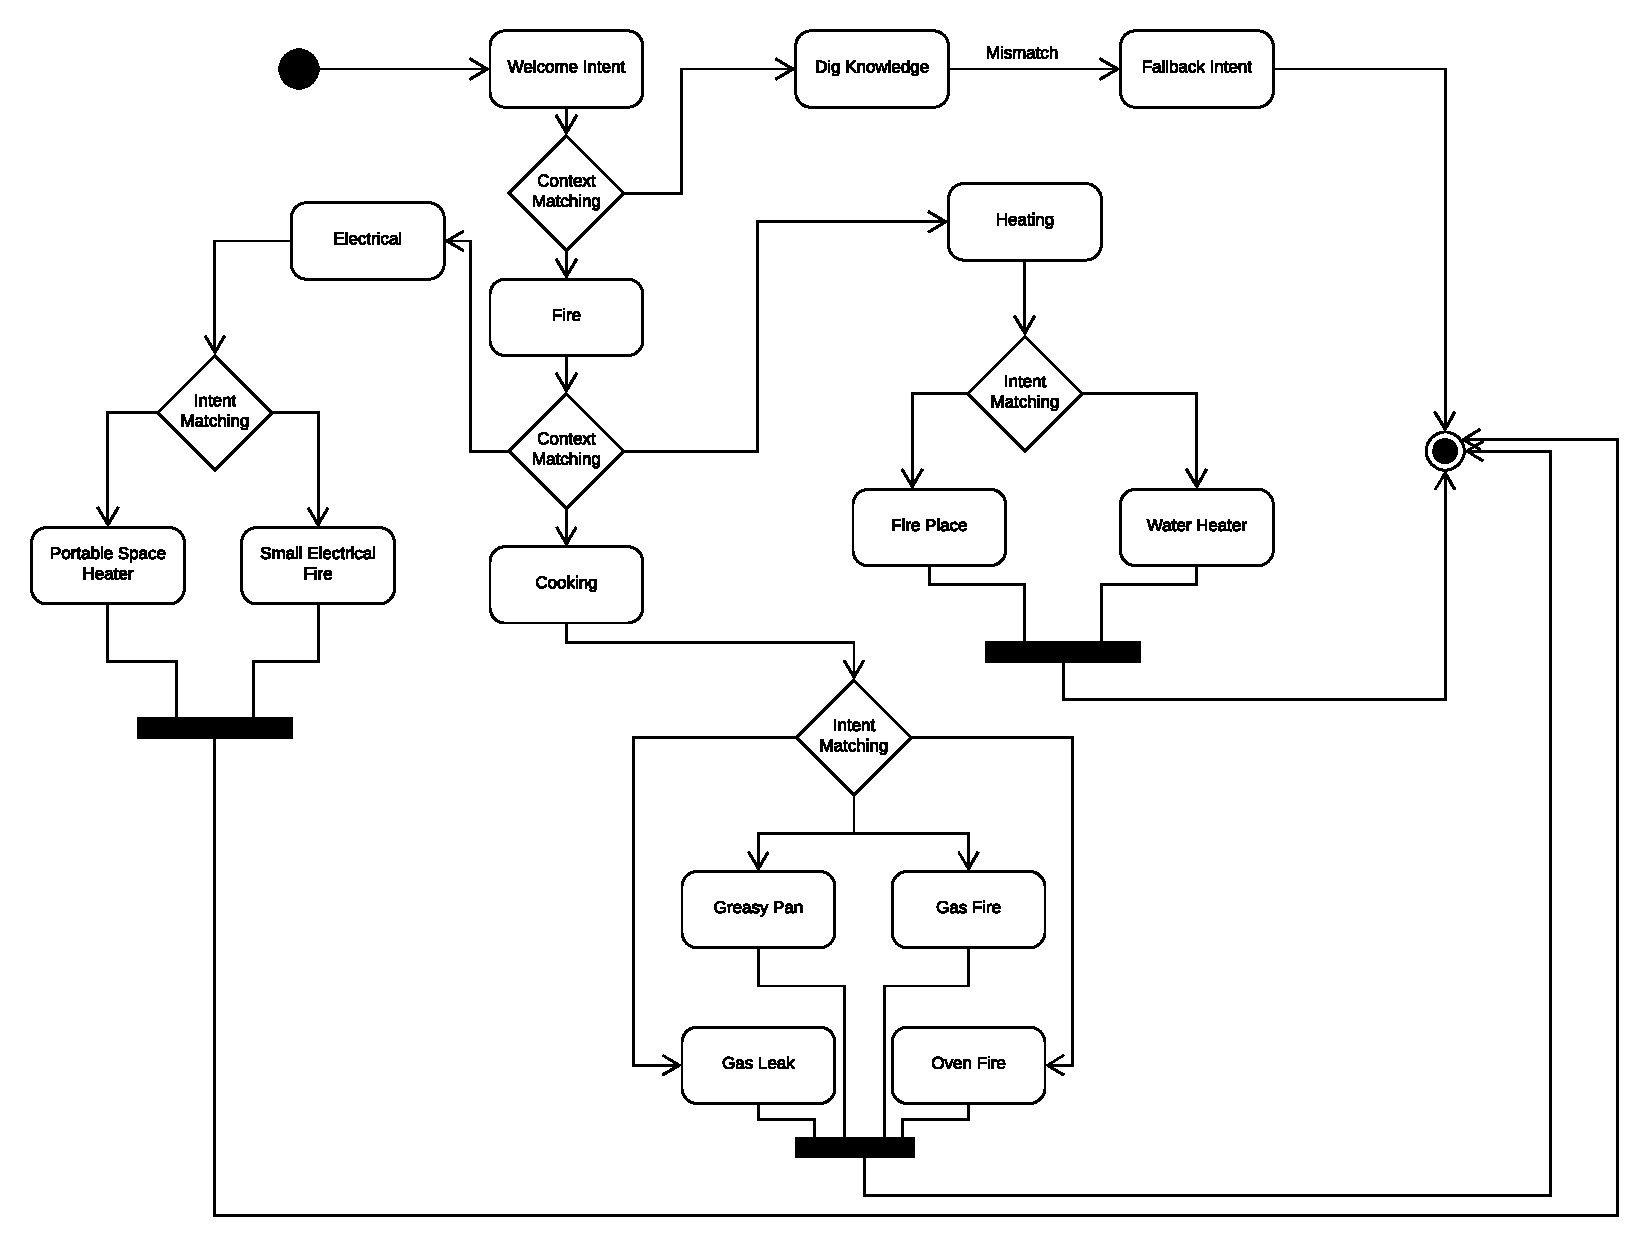
\includegraphics[angle=90, width=.95\textwidth]{img3/state2.pdf}
    \caption{State Chart Diagram - Context Matching (cont.)}
    \label{fig:statechartdiagram2}
\end{figure}

\clearpage
\begin{figure}[ht!]
    \centering
    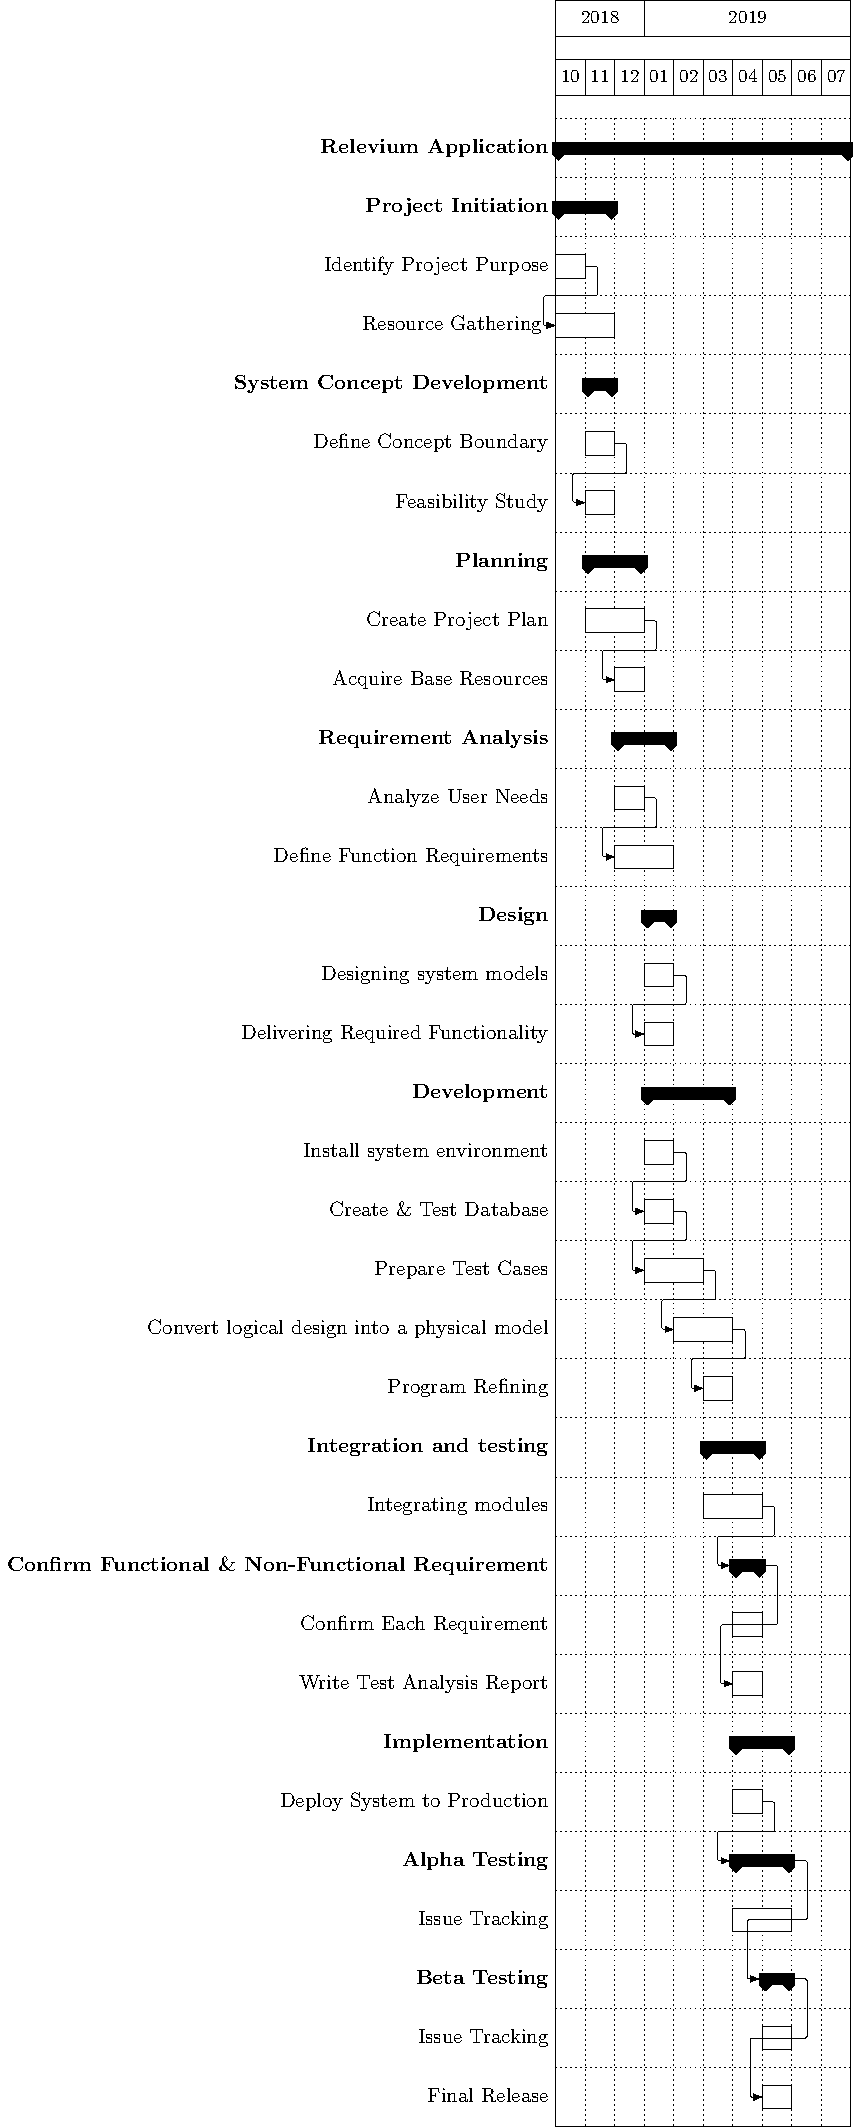
\includegraphics[height=\textheight]{gantt/gantt_month.pdf}
    \caption{Gantt Chart - Simple View}
    \label{fig:gantt1}
\end{figure}

\clearpage
\begin{figure}[ht!]
    \centering
    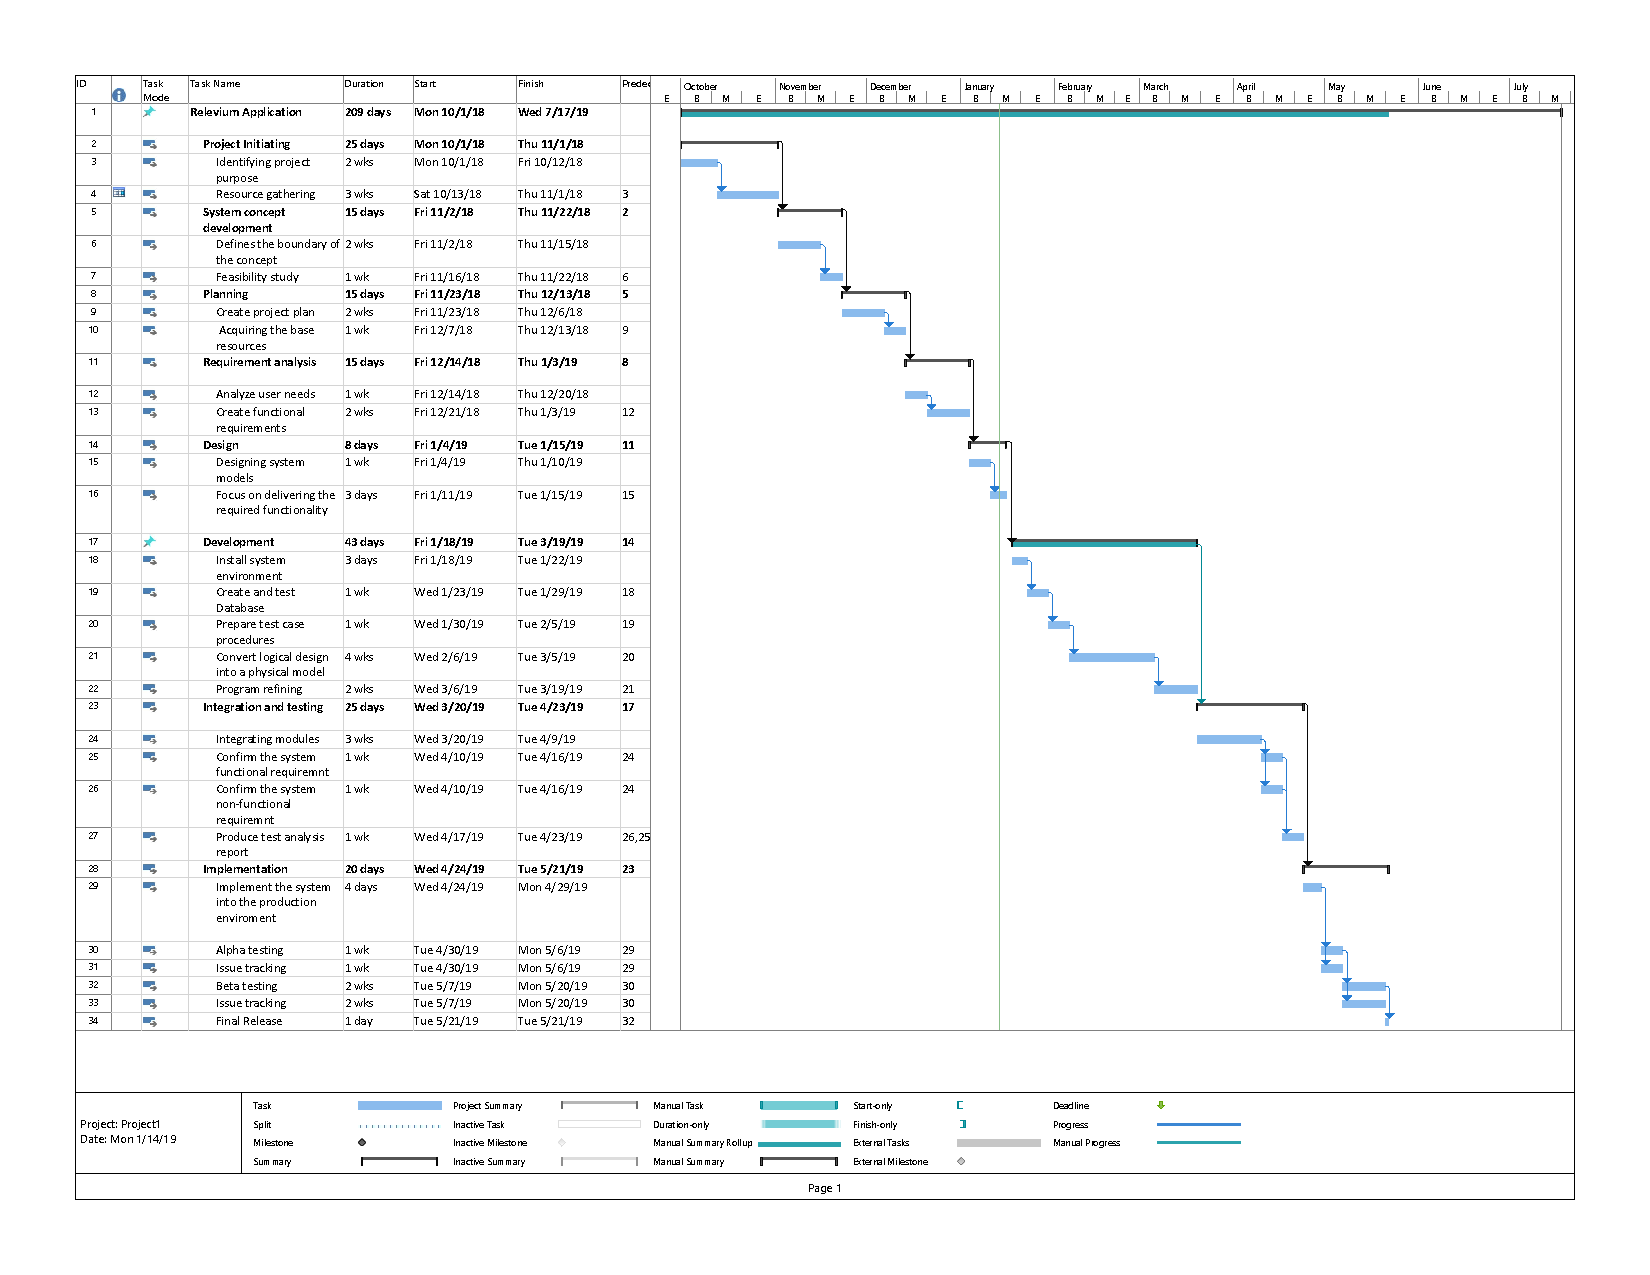
\includegraphics[angle=90, height=\textheight]{gantt/gantt_scale.pdf}
    \caption{Gantt Chart - Detailed View}
    \label{fig:gantt2}
\end{figure}






% \section{Appendix A: Glossary}
% %see https://en.wikibooks.org/wiki/LaTeX/Glossary
% $<$Define all the terms necessary to properly interpret the SRS, including 
% acronyms and abbreviations. You may wish to build a separate glossary that spans 
% multiple projects or the entire organization, and just include terms specific to 
% a single project in each SRS.$>$

% \section{Appendix B: Analysis Models}
% $<$Optionally, include any pertinent analysis models, such as data flow 
% diagrams, class diagrams, state-transition diagrams, or entity-relationship 
% diagrams.$>$

% \section{Appendix C: To Be Determined List}
% $<$Collect a numbered list of the TBD (to be determined) references that remain 
% in the SRS so they can be tracked to closure.$>$

\end{document}